\chapter{Introduction to Dark Matter}
\label{chap:chap1}

%% Restart the numbering to make sure that this is definitely page #1!
\pagenumbering{arabic}

Ever since humankind harnessed the capacity for curiosity, the universe, along with everything it holds has become a vast playground in which the game is to look outwards into the depths of the universe and inwards into the depths of the fabric, the fundamental building blocks of the universe. The introduction of general relativity, followed by the observations of Edwin Hubble lead to a picture of the universe that's non-static and ever expanding. Soon after, dynamical studies of galaxies and galaxy clusters by Fritz Zwicky unfolded a discrepancy between the expected luminous mass and inferred mass of such clusters \cite{Fritz_Zwicky_1993}. The presence of "dark" or unseen matter in galaxies was suggested by a variety of different techniques thereafter. Although unseen, the gravitational influence of dark matter is apparent in many facets of cosmology, leading to a universe that's predominantly dark in matter density and undiscovered. This chapter will explore the theoretical and observational motivations for dark matter, delving into the different candidates to explain it's nature and introducing the Weakly Interacting Massive Particles, one of the leading candidates for dark matter. 

%%------------------------------$$
\section{Modern Cosmology}
\label{sec:moderncosmology}

Our modern understanding of the universe emerged with key cosmological observations and realisations at the start of the 20th century. The measurement of the first Doppler shift of the Andromeda galaxy in 1913 and the subsequent measurements made by Vesto Slipher, although controversial at the time, showed that almost all such galaxies were receding from Earth \cite{Slipler}. The expanding universe hypothesis was further strengthened by Georges Lemaître and Alexander Friedmann in the 1920s when they independently used Einstein's field equations to showed that the universe may be expanding \cite{Friedman}. But this hypothesis gained most of it's attraction when Erwin Hubble that showed the correlation between distant galaxies and their recession velocities---dubbed as Hubble's Law \cite{Hubble}.


%%----------------$$
\subsection{The Expanding Universe}

The spectral light from distant stars in galaxies outside of our local group appear to be shifted as these galaxies move away from Earth. Interpreted as the Doppler effect in flat spacetime, the velocity $v$ related to the shift in  spectral wavelength $\Delta \lambda/\lambda$ is given by the Doppler formula,
%
\begin{equation}
  v/c = \Delta \lambda/\lambda \equiv z,
\end{equation}
%
for $V \ll c$, where $z$ is the astronomical definition of redshift. 

Erwin Hubble showed that for galaxies sufficiently close, where their distance can be measured, the velocity $\vec{v}$ of these galaxies and their distance $\vec{r}$ followed a simple linear relationship, called Hubble's law:
%
\begin{equation}
  \boldsymbol{\vec{v}} = H_0\boldsymbol{\vec{r}}.
\end{equation}
%
The constant of proportionality, $H_0$ is called the Hubble constant. The Hubble constant represents the present day expansion rate of the universe and is usually given with a dimensionless parameter $h_0$, where
%
\begin{equation}\label{eq:hubble_constant}
  H_0 = 100h_0 \; \MathText{km} \; \MathText{s}^{-1} \; \MathText{Mpc}^{-1}, \; \MathText{where} \; h_0 = 0.674 \pm 0.005 \: \cite{Plank_2018}.
\end{equation}
%

Hubble's law is a phenomenological relationship between redshift and distance, implying that the further a galaxy is, the faster it is moving away from us. The law holds for galaxies that are far enough away that any velocity disruptions due to local gravitational effects are subdominant to the expansion rate. While at the same, these galaxies cannot be too far away that the effects of spacetime curvature or the expansion of the universe in the time it takes for the photons to travel become significant. 

The expansion of the universe leads to the concept of the expansion of space. The expansion is often represented in co-moving coordinates $\boldsymbol{\vec{x}}$. The distance associated with the expansion---the co-moving distance---is a time independent measure between two fundamental observers. In a universe that's expanding under isotropy and homogeneity, the physical distance or proper distance $\boldsymbol{\vec{r}}$ is related to the co-moving coordinates moving along with the expansion of space by
%
\begin{equation}
  \boldsymbol{\vec{r}} = a(t)\boldsymbol{\vec{x}},
\end{equation}
%
where $a(t)$ is the time-dependent cosmological scale factor, representing the change in distance between two fundamental observers due to the expansion.

Differentiating $\boldsymbol{\vec{r}}$ with respect to time leads to the recession velocity $\boldsymbol{\vec{v}}$ of an observer or a galaxy in the same direction as its displacement away from earth, where
%
\begin{equation}
  \boldsymbol{\vec{v}} = \dv{\boldsymbol{\vec{r}}}{t} \equiv  \dot{a(t)}\boldsymbol{\vec{x}},
\end{equation}
%
leading to the relationship,
%
\begin{equation}
  H(t) = \frac{\dot{a(t)}}{a(t)}.
\end{equation}
%
The equation above gives the connection of the Hubble constant to the geometry of spacetime, where $H(t)$ is the time-dependent Hubble parameter, defining the relative expansion of space. The Hubble constant $H_0$ we measure is $H(t)$ at the present time of the universe.

The expansion of space requires a time-dependent geometry in which a particle's energy moving through this geometry will change similar to it moving through a time-dependent potential. A photon whose energy is proportional to frequency and therefore its wavelength, will experience the expansion as a stretch in its wavelength. This cosmological redshift is defined in terms of the scale factor as
%
\begin{equation}
  z \equiv \frac{\lambda(t_0) - \lambda(t)}{\lambda(t)} = \frac{\lambda(t_0)}{\lambda(t)} -1 = \frac{a(t_0)}{a(t)} - 1,
\end{equation}
%
where $t$ represents cosmic time and $t_0$ present time.

The Hubble constant has the dimensions of an inverse time. The inversion is called the Hubble time $t_H$. In a version of the universe in which $\ddot{a(t)} \leq 0$, the Hubble time becomes an upper bound and a rough estimate of the age of the universe, placing the age to $\sim$ 14 billion years. With the cosmological observations of this era, the picture of the universe moved towards one in which the universe had a beginning and from that start came the expansion. But the Hubble expansion alone does not provide sufficient evidence and description for what is generally refer to as the hot Big Bang model of cosmology. The description comes from the application of the cosmological principle to Einstein's theory of General Relativity.

%%----------------$$
\subsection{Cosmological Principle}
\label{subsec:cosmological_principle}

The dynamics of the universe are governed by the Einstein field equation, relating the curvature of spacetime to density of mass-energy \cite{Gravity}
%
\begin{equation}\label{eq:einstein_field_eq}
  R_{\mu\nu} - \frac{1}{2} g_{\mu\nu}R + g_{\mu\nu}\Lambda = \frac{8\pi{}G}{c^4} T_{\mu\nu},
\end{equation}
%
where $R_{\mu\nu}$ is the Ricci curvature tensor, R is the scalar curvature, $g_{\mu\nu}$ is the metric tensor, $\lambda$ is the cosmological constant, $G$ is gravitational coupling constant and $T_{\mu\nu}$ is the stress–energy tensor. The left hand side of this equation describes the geometrical structure of spacetime and the right describes the measure of matter and energy density of the Universe. The cosmological constant $\Lambda$ was originally introduced by Einstein as a tuning mechanism for a static cosmology with non-zero matter content but later interpreted as the energy density of the vacuum, a source of energy and momentum that may be present in the absence of matter fields \cite{SeanC}.

Modern cosmology for some time has relied upon the premise offered by the cosmological principle. This principle states that the Universe on large scales is homogeneous and isotropic, where local variations in density are averaged over. A homogeneous, isotropic spacetime is one for which the geometry is spherically symmetric about any one point (isotropic) and the same in all points (homogeneous). Although isotropy and homogeneity is assumed for space, when we look at distant galaxies, they appear to be receding from us; the universe is apparently not static, but changing with time. Therefore, any cosmological model of the universe must assume a homogeneous and isotropic universe in space but not in time. Spacetime can therefore be considered as $\boldsymbol{T} \cross U$, where $\boldsymbol{T}$ represents the time direction and $U$ is a homogeneous and isotropic three-manifold. The usefulness of homogeneity and isotropy is that they imply that $U$ must be a maximally symmetric space, taking the form of a metric
%
\begin{equation}
    ds^2 = -dt^2 + a^2(t)\gamma_{ij}(u)du^2du^j,  
\end{equation}
%
where $t$ is the timelike coordinates, ($u^1, u^2, u^3$) are the coordinates on $U$ and $\gamma_{ij}$ is the maximally symmetric metric on $U$. The dimensionless scale factor $a(t)$ is a function of proper time $t$, representing the scale of the space-like slice of spacetime at the present moment.

The geometrical interpretation of the cosmological principle can be shown to take a similar form to that of equation (\ref{eq:einstein_field_eq}) as the Friedmann-Robertson-Walker (FRW) metric---a metric tensor which describes a homogeneous and isotropic spacetime that evolves as a function of time (see \cite{Modern_Cosmology, Gravity} for an in-depth review). The three line elements of the metric tensor can be written in a unified form to give the well known FRW metric,
%
\begin{equation}
  ds^2 = -dt^2 + a^2(t) \left[ \frac{dr^2}{1 - kr^2} +r^2(d\theta^2 + sin^2\theta d\phi) \right],
\end{equation}
%
where \textit{r}, \theta and \phi represent the co-moving polar coordinates. The parameter \textit{k} represents the curvature of the universe, where +1, 0, -1 is for a closed, flat or an open universe respectively, corresponding to a positive, zero or a negative curvature of space.

The FRW model assumes a cosmological fluid consisting of three non-interacting components: pressureless matter, relativistic particles \& radiation and vacuum. This can be modelled by an energy-momentum tensor of a perfect fluid, specified by an energy density $\rho$  and isotropic pressure $p$ as 
%
\begin{equation}\label{eq:em_tensor}
  T_{\mu\nu} = (\rho + p)u_{\mu}u_{\nu} + pg_{\mu\nu}, 
\end{equation}
%
where $u^{\mu}$ is the fluid four-momentum. Under the boundaries imposed by the cosmological principle, whereby the energy-momentum tensor takes the form of a perfect fluid (\ref{eq:em_tensor}), the Einstein field equation (\ref{eq:einstein_field_eq}) reduces to the Friedmann equations \cite{Friedman, SeanC}:
%
\begin{equation}
  H^2 \equiv \left( \frac{\dot{a}}{a} \right)^2 = \frac{8\pi{}G}{3}\rho - \frac{kc^2}{a^2} + \frac{\Lambda}{3}
\end{equation}
%
%
\begin{equation}\label{eq:friedmann_2}
    \frac{\ddot{a}}{a} = -\frac{4\pi{}G}{3}(\rho + 3p) + \frac{\Lambda{}c^2}{3}.
\end{equation}
%
Examining these equations under certain assumptions can lead to useful cosmological quantities. In assuming a flat spacetime, where spatial curvature $k=0$ and one which is static ($\Lambda = 0$), leads to the quantity known as the critical density, 
%
\begin{equation}\label{eq:crit_density}
  \rho_{crit} \equiv \frac{3H^2(t)}{8\pi{}G} \simeq 1.88 \times 10^{-29} \: h^2 \: \MathText{g cm}^{-3} \: \cite{pdg}.
\end{equation}
%
The cosmological density parameter, a useful definition in comparing different cosmological models is then defined as
%
\begin{equation}\label{eq:omega_tot}
  \Omega_{tot} = \frac{8\pi{}G}{3H^2}\rho = \frac{\rho}{\rho_{crit}}.
\end{equation}
%
Under the conditions where $\Lambda = 0$ and by using (\ref{eq:omega_tot}), the Friedmann equation (1.12) can be shown to take the form
%
\begin{equation}\label{eq:density_param}
  \Omega_{tot} - 1 = \frac{kc^2}{a^2H^2}, 
\end{equation}
%
where the sign of spacetime curvature parameter $k$ is determined by whether $\Omega_{tot}$ is greater than, equal to, or less than one. This reduction leads to a picture in which $\rho < \rho_{crit}$, $\rho = \rho_{crit}$ and $\rho > \rho_{crit}$, equate to a universe that is respectively open ($k=-1$), flat ($k=0$) or closed ($k=+1$). 

The observational determination of the density parameter is an area of intense investigation and it is often necessary to distinguish different contributions to the overall density. One can conveniently define the present-day density parameters for pressureless matter as $\Omega_{m}$, relativistic particles and radiation as $\Omega_r$ and the quantity $\Omega_{\Lambda} = \Lambda/3H^2$. Thus, the total density of the universe may be defined as, 
%
\begin{equation}
  \Omega_{tot} = \Omega_{r} + \Omega_{m} + \Omega_{\Lambda}. 
\end{equation}
%
The Friedmann equation then takes the form
%
\begin{equation}
  \frac{kc^2}{a_{0}^2H_{0}^2} = \Omega_{r} + \Omega_{m} + \Omega_{\Lambda} - 1
\end{equation}
%
where the subscript 0 indicates present day values. 

The conclusion one takes is that the curvature of space denoted by the left side of the equation depends on the sum of densities in matter, relativistic particles, and vacuum.  The $\Omega_{tot}$ parameter as given in (\ref{eq:density_param}), plays an important role in the evolution of universe through its gravitational potential. The observational determination of the density parameter and its constituents will highlight which of the three Robertson-Walker geometries describes our universe. In a simplified scenario in which $\Lambda = 0$ and universe is filled with fluids of positive energy ($\rho > 0$) and non-negative pressure ($p \geq 0$), equation (\ref{eq:friedmann_2}) leads to $\ddot{a} < 0$. Since the expansion of the universe is verified by the motion of distant galaxies, where $\dot{a} > 0$, this leads to the conclusion that the rate at which the universe is expanding is negative, hence the expansion is decelerating. This is as expected, since the gravitational attraction of the matter content of the universe works against expansion. In tracing the evolution backwards in time, a singularity is reached at $a = 0$. If $\ddot{a}$ were exactly zero, the age of the universe would be $H_{0}^{-1}$. The singularity represents a point in which the universe began from a singular state and this point in history is commonly known as the "big bang".  


%%------------------------------$$
\section{Evidence for Dark Matter}
\label{sec:darkmatter}

The evolution of the universe is governed by the total density content and from which, the interplay between the matter, radiation and vacuum densities. The cosmic inflation theory requires a universe that is flat, hence $\Omega_{tot} = 1$. With the premise that the universe is flat and by taking into account complementary theoretical and experimental techniques, it becomes possible to quantify the matter density of the universe. By examining the universe on  different cosmological scales via Big Bang Nucleosynthesis (BBN), the Cosmic Microwave Background (CMB) and Gravitational Lensing, a picture emerges in one which roughly 95\% of the total energy density of the universe still lacks scientific exploration and largely remains a mystery. This section will examine some of the leading cosmological and astronomical observations in more detail, concluding that the levels of observed or luminous matter in the universe does not account for the total matter and that the majority of the matter content of the universe is non-baryonic and non-luminous. 

\subsection{Cosmic Microwave Background}
\label{subsec:CMB}

The cosmic microwave background radiation, first discovered in mid-1960s \cite{CMB_disc}, is thought of as a primordial radiation from the early universe. In the hot Big Bang model, the early universe is extremely hot and dense, leading to a constant scattering of particles and radiation. At around a redshift ~1100 and roughly 380,000 years of age, the expansion of space cooled the plasma, allowing the first atoms to form through recombination, effectively decoupling the radiation from matter and making the universe transparent to photons. The collisions of these photons with electrons before last scattering ensures that the photons were in equilibrium. Travelling freely through space, this radiation is still present today but has been redshifted due to the expansion of the universe. The CMB photons are detected on earth with a spectral distribution that of a black body function with $T = 2.725$ K \cite{cmb_temp}. The CMB as observed from earth is roughly homogeneous and isotropic but at scales of around $10^{-6}$, it contains small temperature fluctuations (or anisotropies). The most detailed observation to-date of the CMB anisotropies comes from the Planck collaboration \cite{plank_cmb_map}, where an all sky map of the temperature anisotropies measured by their space observatory is shown in figure (\ref{fig:cmb_map}).

\begin{figure}[ht!]
    \begin{center}
        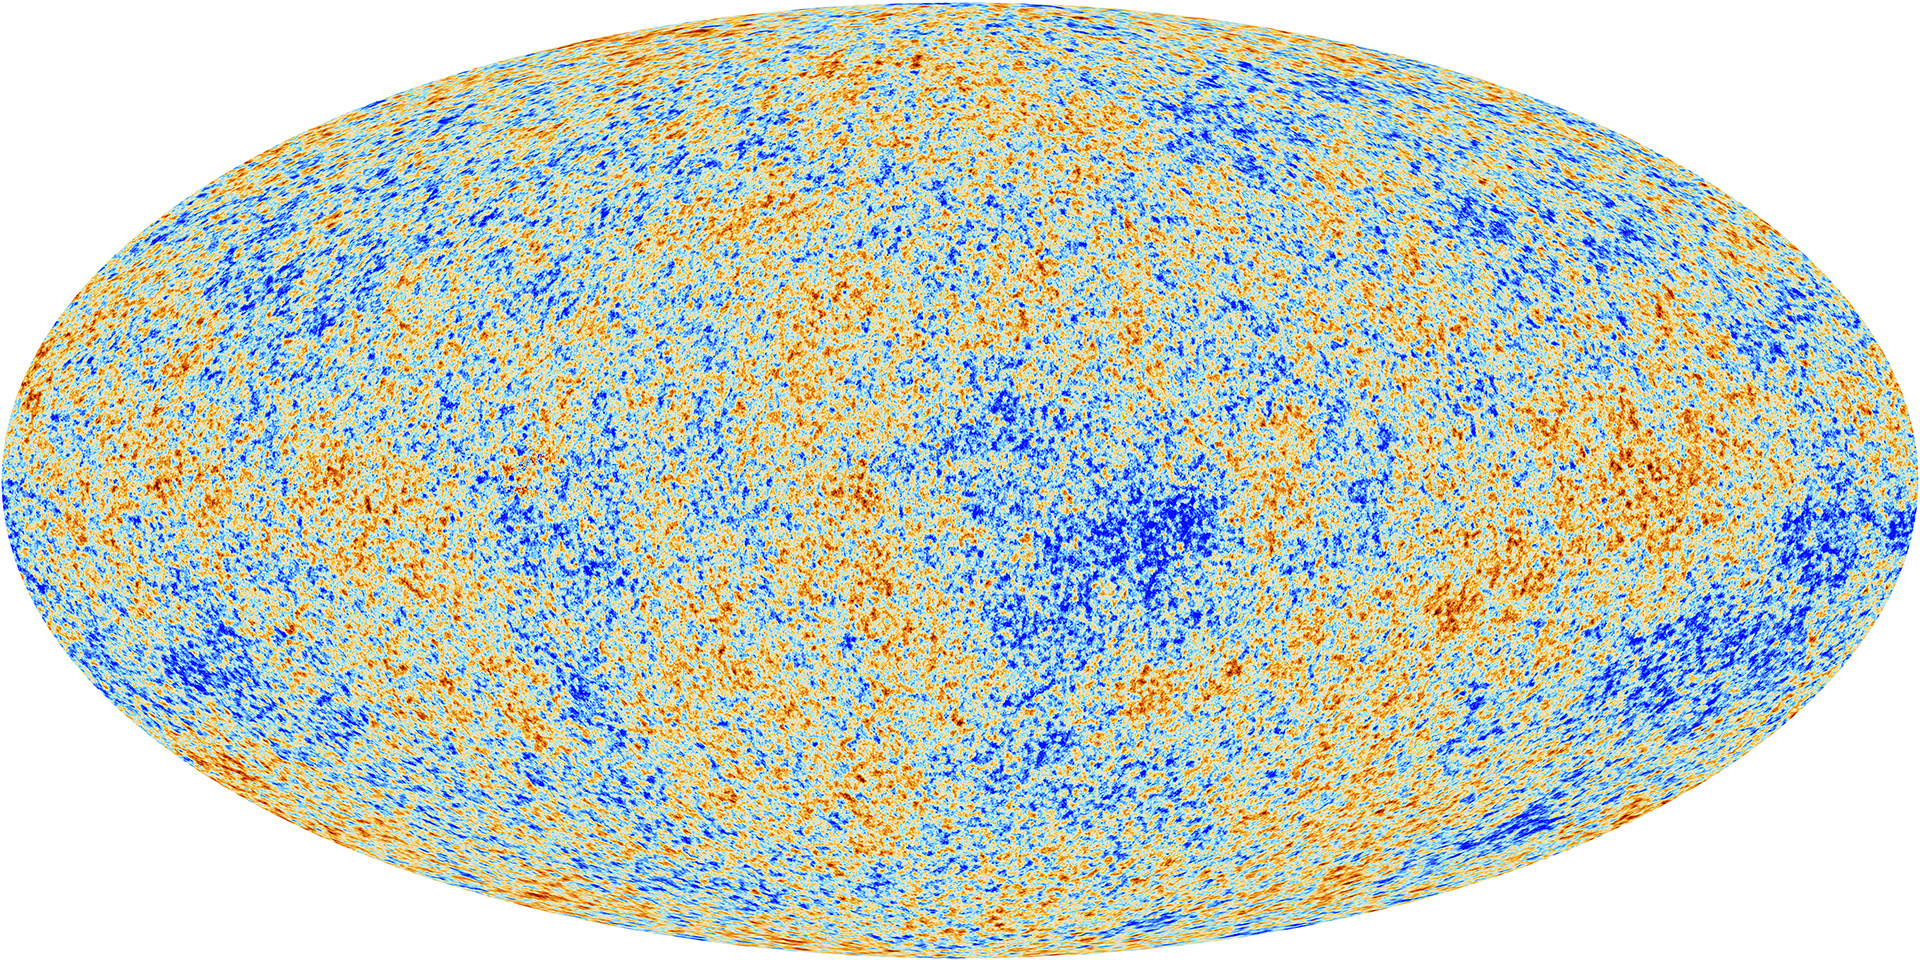
\includegraphics[scale=0.2]{Chapter_1/Figures/Planck_CMB.jpg}
        \caption[The map of the all sky CMB radiation as illustrated by the Planck collaboration, showing in detail the temperature anisotropies.]%
        {The map of the all sky CMB radiation as illustrated by the Planck collaboration, showing in detail the temperature anisotropies. The temperature difference between blue and red in the figure is a few thousandths of a Kelvin and correspond to matter density fluctuations in the distribution.}
        \label{fig:cmb_map}
        \end{center}
\end{figure}

The anisotropies observed in the CMB can be mapped at different angular scales. These angular scales are representations of the physical size of anisotropies at the time of the last-scatter. The angular scales of the fluctuations can be parametrised as the multipole moments ($l$) of a spherical harmonic, which determines the wavelength, $\lambda = 180\circ/l$ of the mode on the sphere of the CMB. The mapping of the different scales are given as the power spectrum of the CMB and shown in figure (\ref{fig:cmb_power_spectrum}).

\begin{figure}[ht!]
    \begin{center}
        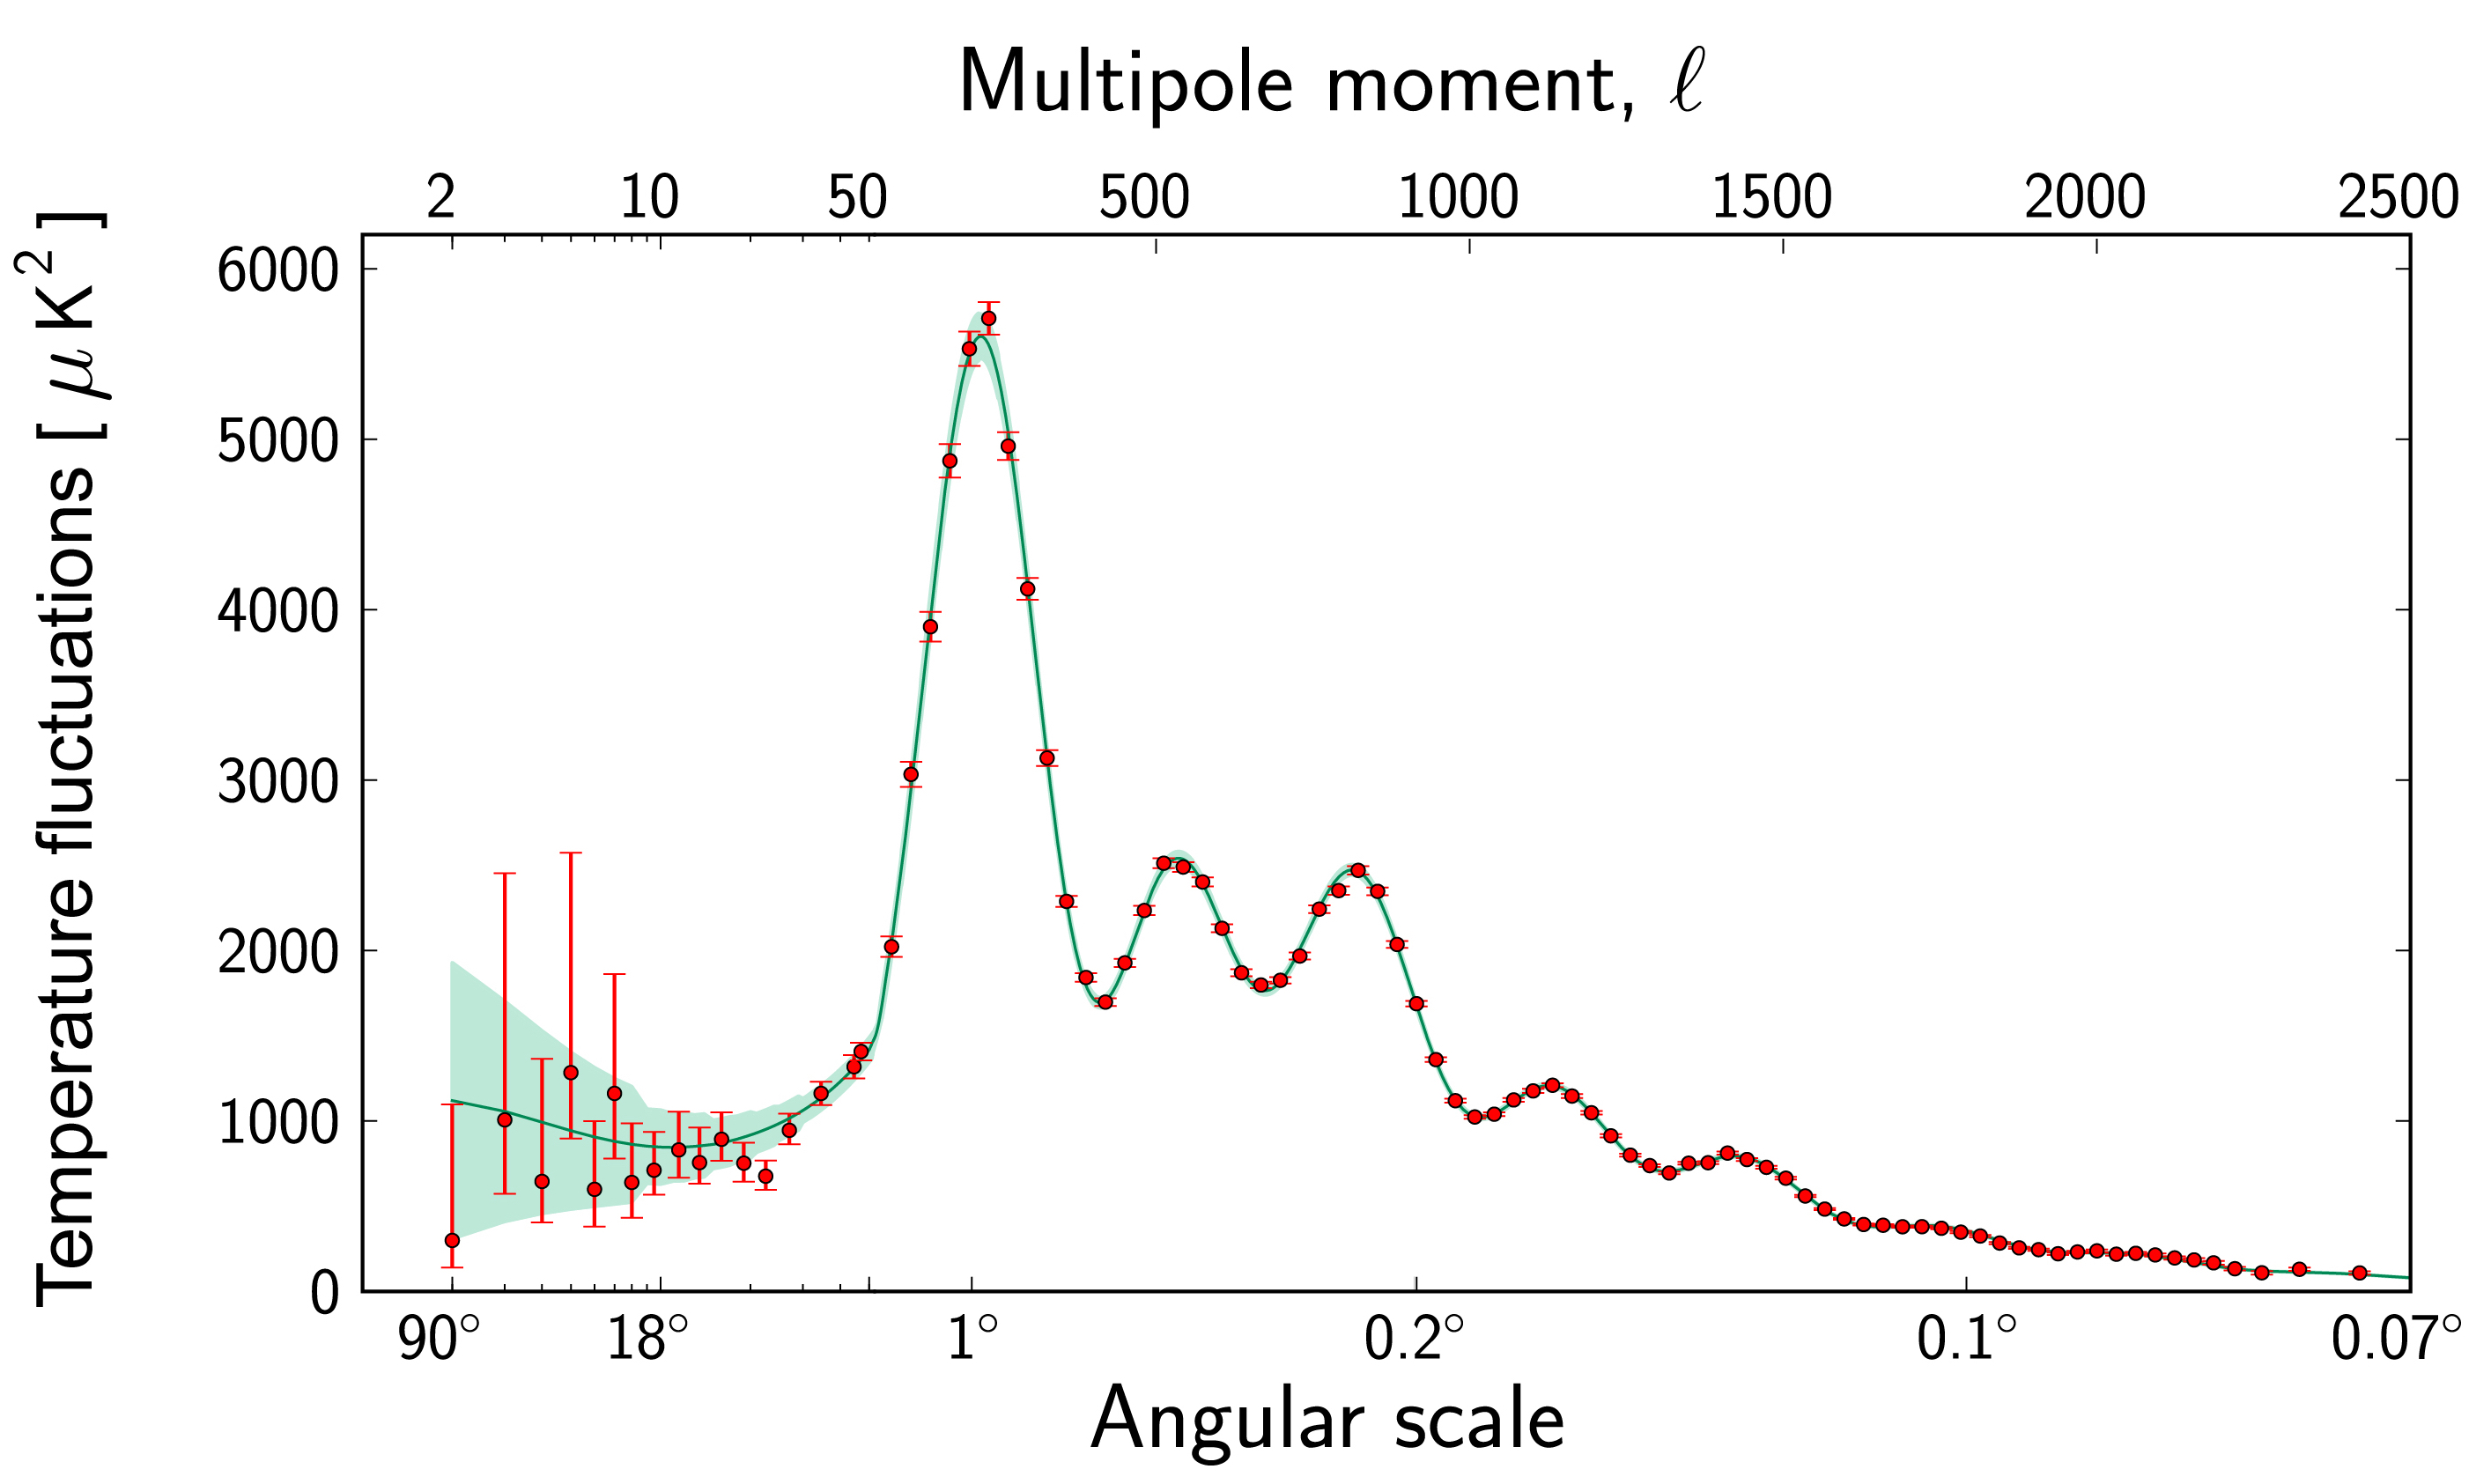
\includegraphics[scale=0.15]{Chapter_1/Figures/Planck_power_spectrum.jpg}
        \caption[The map of the all sky CMB radiation as illustrated by the Planck collaboration, showing in detail the temperature anisotropies.]%
        {The angular power spectrum of the CMB temperature fluctuations as measured by Planck. The green line fitted onto the seven acoustic peaks is the six-parameter $\Lambda$CDM model. The shaded area around the best-fit curve represents cosmic/sample variance, including the sky cut used.}
        \label{fig:cmb_power_spectrum}
        \end{center}
\end{figure}

The primary anisotropies of the CMB are due to the last scattering of photons in the recombination epoch. Perturbations in the primordial plasma lead to collapse of matter in regions of over-density. The gravitational collapse lead to an increase in radiation pressure of the photon-baryon plasma, which eventually counteracted local gravitational wells and set up acoustic oscillations. Photons from high-density regions at last scattering were redshifted climbing out of these potential wells. Furthermore, adiabatic fluctuations in these regions lead to an increase in temperature. and velocity fluctuations within the plasma would have further resulted in Doppler shifts in frequency. The peaks observed in the power spectrum correspond, roughly, to resonances in which the photons decouple when a particular mode is at its peak amplitude.

The ability to probe and image the very early universe via the CMB at the moment of recombination opens the way to understand, model and extract information about the contents of the early universe. The amplitudes and positions of the peaks observed in the power spectrum are dependent on the baryonic and non-baryonic matter content of the early universe, and on the geometry of space. Since light propagates along geodesics in space and the size of the horizon at recombination can be inferred by the properties of the plasma, the geometry of space can then be determined by the understanding of the the expansion history. A flat space-time corresponds to a first peak around $l$ of \sim220. The higher order peaks of the spectrum can provide information on the baryonic and non-baryonic matter densities in the early universe. In particular the third peak is sensitive to the density ratio of matter to radiation. The dampening observed as $l$ increased is due to the washing out of fluctuations initially set by inflation. The third peak, however is boosted relative to the rest, demonstrating the domination of matter in the plasma before the time of recombination and encapsulates the information present on the dark matter content of the early universe.

The power spectrum of the CMB is well described by the Lambda Cold Dark Matter ($\Lambda$CDM) model as shown in (\ref{fig:cmb_power_spectrum}). $\Lambda$CDM emerged as the standard model of cosmology in describing the evolution of the universe with its matter content \cite{Modern_Cosmology}. In explaining and parametrising the Big Bang cosmological model, $\Lambda$CDM requires a cosmological constant ($\Lambda$)---associated with the vacuum energy contribution or also known as dark energy, and the presence of ordinary and non-baryonic Cold Dark Matter (CDM). In fitting this model to the power spectrum, Planck extracts some of the density parameters defined in section (\ref{subsec:cosmological_principle}), where $\Omega_{\Lambda} =  0.6847 \pm 0.0073$ and $\Omega_{m} =  0.3153 \pm 0.0073$ \cite{Plank_2018, Plank_2018_2}. Furthermore, Planck extracts the baryon and cold dark matter densities from the $\Lambda$CDM model fit parameters to give $\Omega_{b}h^2 = 0.02237 \pm 0.00015$ and $\Omega_{c}h^2 = 0.1200 \pm 0.0012$. Normalising these with the the Hubble constant given in equation (\ref{eq:hubble_constant}) results in $\Omega_{b} \sim 0.049$ and $\Omega_{CDM} \sim 0.265$. The information captured by the CMB and its power spectrum points towards a universe that is \sim 68\% dark energy and \sim 32\% matter. The non-baryonic cold dark matter further contributes to \sim 84\% the total matter content of the universe.


\subsection{Big Bang Nucleosynthesis}
\label{subsec:BBN}

The radiation temperature of the universe moments after the big bang were above the MeV binding energies of nuclei and way above the KeV binding energies of atoms. Any nuclei or atom present would have quickly disintegrated into electrons, protons and neutrons. Within the first few minutes, when the temperatures dropped below nuclear binding energies, nuclear reactions lead to the formation of the very first nuclei via the process known as Big Bang Nucleosynthesis. The relative primordial abundance of isotopes such as D, $^{3}$He, $^{4}$He and $^{7}$Li synthesised minutes after the big bang and depend on the cosmological parameters of the universe \cite{pns}. 

As the baryon number is conserved at and below MeV temperatures, the process of nucleosynthesis and the abundance of primordial isotopes depend on the total baryon number and thus $\Omega_{b}$ in the early universe. The relative abundances can be measured today in places such as old stars, low mass local galaxies and the edges of distant galaxies, where a small change in primordial abundance is presumed. The primordial abundances of D, $^{3}$He, $^{4}$He and $^{7}$Li as predicted by the standard model of Big-Bang nucleosynthesis is shown in figure (\ref{fig:primordial_abundance}). The figure shows the theoretical dependency of primordial isotopic ratios on the baryon/photon ratio (\eta) in the early universe and by extension, on $\Omega_{b}$.

\begin{figure}[ht!]
    \begin{center}
        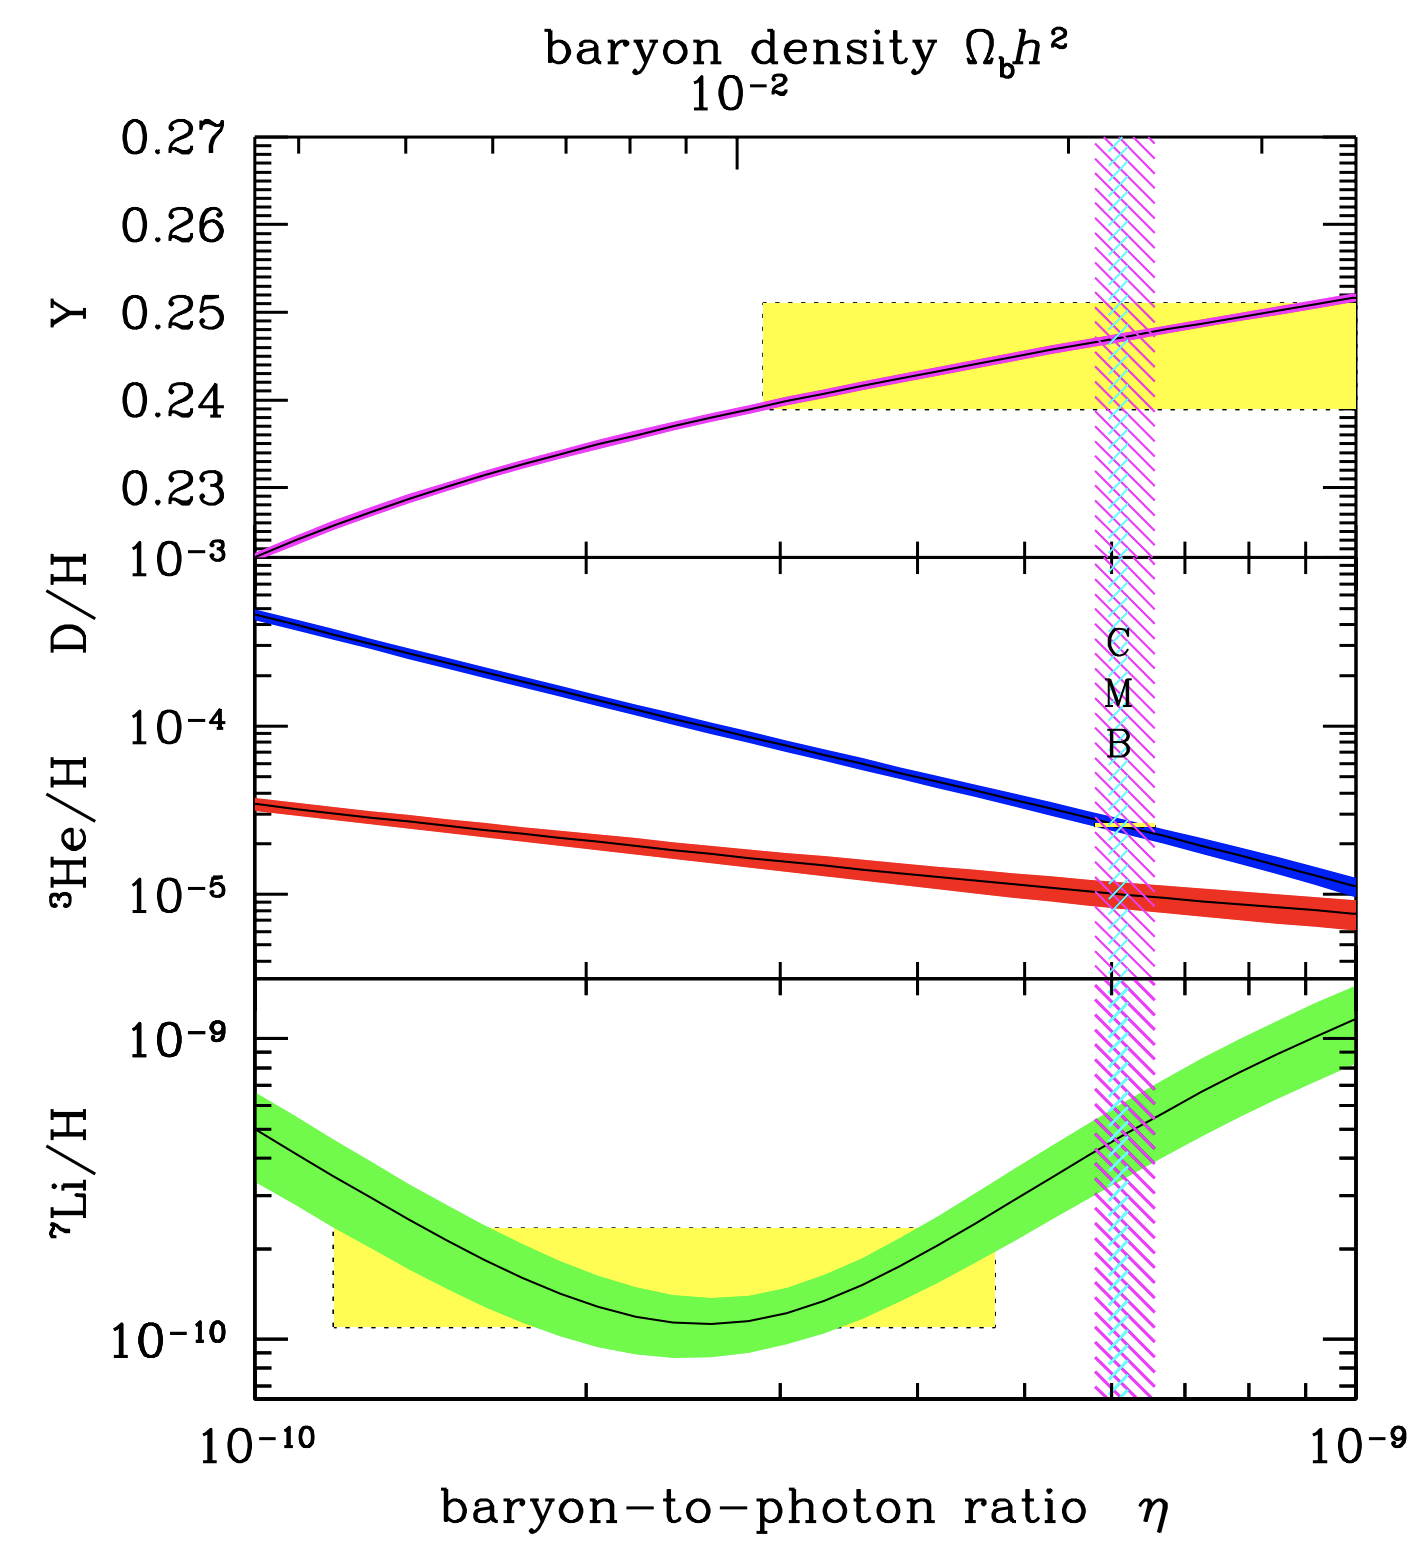
\includegraphics[scale=0.45]{Chapter_1/Figures/BBN_primordial_abundance.jpg}
        \caption[The primordial abundances of $^4$He, D, $^3$He, and $^7$Li as predicted by the standard model of Big-Bang nucleosynthesis]%
        {The primordial abundances of $^4$He, D, $^3$He, and $^7$Li as predicted by the standard model of Big-Bang nucleosynthesis with the bands highlighting the 95\% CL range. Yellow boxes indicate the observed light element abundances and the vertical band indicates the CMB measure of the cosmic baryon density \cite{BBN_figure}}.
        \label{fig:primordial_abundance}
        \end{center}
\end{figure}

Deuterium is usually entirely deployed when it is cycled into stars, and the only significant production mechanism is the process of BBN \cite{pns}. Hence, any detection of deuterium provides an upper limit on $\eta_{10}$ and lower limit on the ratio of D/H. The local interstellar value of D/H = $(1.56 \pm 0.40) \times 10^{−5}$ sets a limit of $\eta_{10} < 9$ \cite{d_h_measurements}. Although the \eta range measurements as illustrated by the boxes on figure (\ref{fig:primordial_abundance}) do not all overlap, they are all within a factor of \sim2 from each other. In particular, the discrepancy between the lithium abundance in comparison to the D/H and less-constraining $^4$He abundance is often referred to as the `lithium problem' and could simply reflect the difficulty in determining the primordial lithium abundance (discussed in detail here \cite{Fields_2011}). The measured D/H and $^4$He abundances are in great agreement when the lithium measurement is excluded in due to unknown systematic. The \eta range extracted from the more-precise measurement of D/H gives
%
\begin{equation}
    5.8 \; \leq \; \eta_{10} \; \leq \; 6.6 \; (95\% \; CL),
\end{equation}
%
which provides a measure for the baryon density of the universe as
%
\begin{equation}
    0.021 \; \leq \; \Omega_{b}h^2 \; \leq \; 0.024 \; (95\% \; CL).
\end{equation}
%
Despite the lithium problem, by using only well-established microphysics, the theoretical predictions of the BBN model is in good agreement with both the observations of the D/H abundance and with the baryon density parameter obtained from the CMB by Planck. As an independent observation to that of the CMB, measurements of the primordial isotopic abundances and the BBN model suggest that luminous baryonic matter density $\Omega_{lum} \simeq \Omega_{b}$. This can be seen as further evidence to that obtained from the CMB power spectrum and $\Lambda$CDM, suggesting that the total matter content of the universe cannot be explained by only the presence of baryonic matter alone and the matter density parameter $\Omega_{m} = \Omega_{b} + \Omega_{CDM}$, where a substantial degree of the mass density is comprised of cold dark matter. 

\subsection{Galaxy Rotation Curves}
\label{subsec:rotation_curves}

There is considerable cosmological evidence that most of the mass content of the universe is neither luminous matter nor radiation. Luckily, mass can be detected even if the constituents of this mass is `unseen'. The very early evidence for dark matter comes from studies in the early 1930s, where in studying galaxy cluster dynamics and applying the virial theorem to the coma cluster, Zwicky \cite{Fritz_Zwicky_1993} notice an unusual discrepancy between luminous mass and
estimated mass, making the first claim for unseen matter in galaxies. It wasn't until the 1960s when Ruben and Ford showed further evidence to support Zwicky's claims by studying the rotation curves of starts in spiral galaxies \cite{ruben_ford, ruben_ford_results}.

Galactic scale physics, such as the behaviour of stars orbiting spiral galaxy can readily be explained by Newtonian mechanics. Assuming spherical symmetry, the circular velocity $v_{circ}$ of stars or hydrogen gas clouds orbiting a spiral galaxy at a distance $r$ can be determined using a simple Newtonian relation
%
\begin{equation}
    v_{circ} = \sqrt{\frac{GM(r)}{r}},
\end{equation}
%
where G is the gravitational constant and $M(r)$ is the mass of the galaxy contained within $r$. The relationship above can be written in a form to give the total mass encapsulated up to a specific radius $M(r)$, if the velocities of stars at a distance $r$ can experimentally be obtained. For galaxies that are inclined to the line of sight, spectroscopic radial velocities and radio observations of the 21 cm line of neutral hydrogen at a number of positions on the galactic disc can be used to determine and map out the velocity rotation curves of such galaxies.

\begin{figure}[ht!]
    \begin{center}
        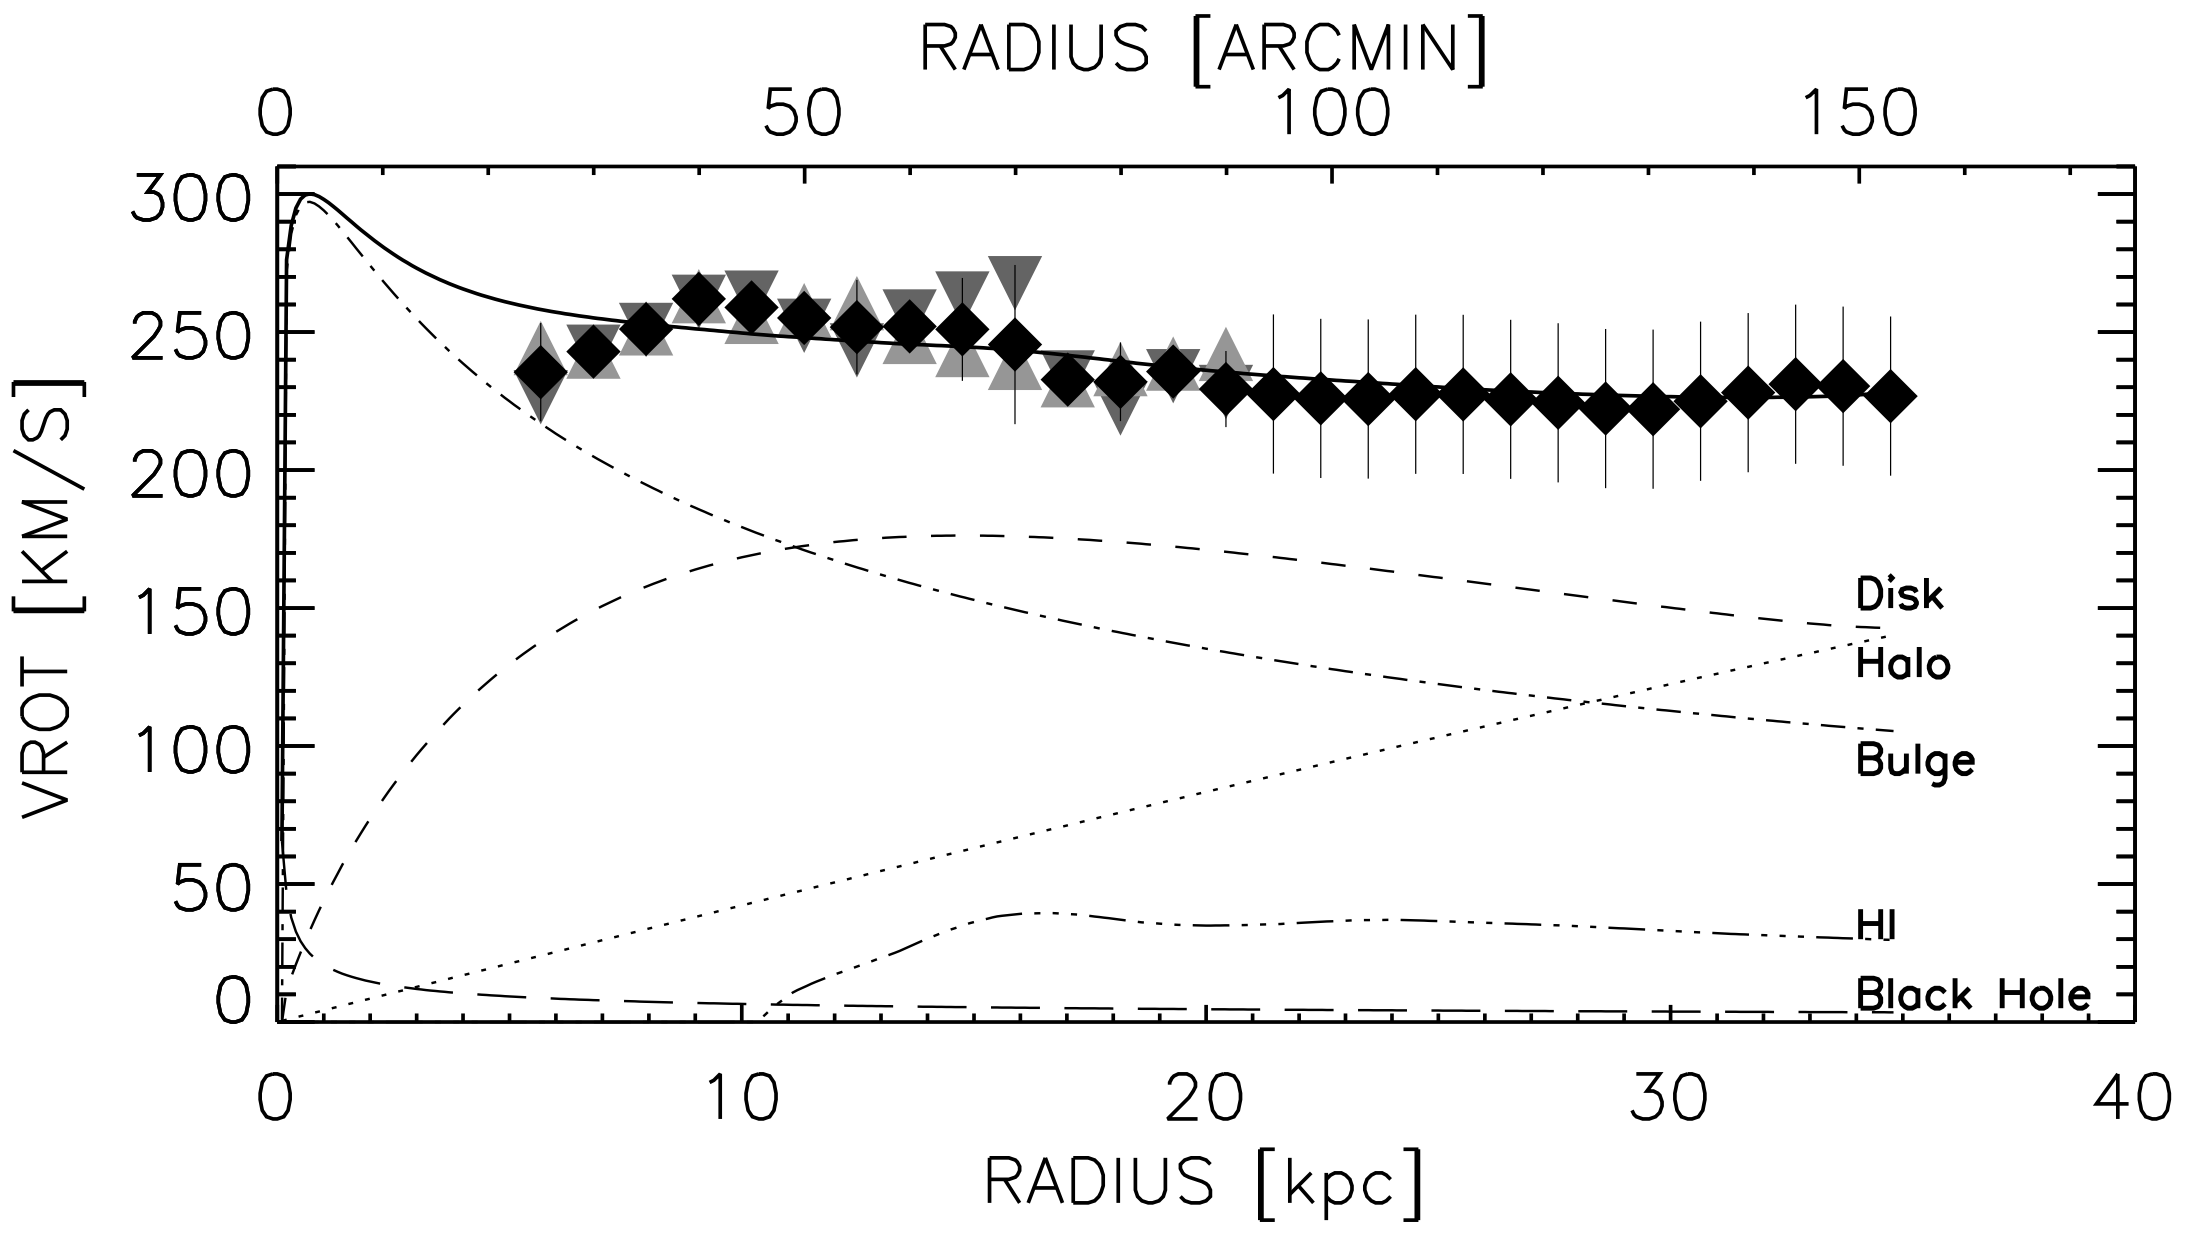
\includegraphics[scale=0.35]{Chapter_1/Figures/Rotation_curve_M31.jpg}
        \caption[Observed rotation curve and corresponding mass models for the Andromeda galaxy (M31) by using data from the Effelsberg and GBT 100 m observations.]%
        {The galactic rotation curve of the Andromeda galaxy (M31) as measured by the Effelsberg and GBT 100 m telescoped. The solid black line represents best fit to data and the corresponding lines below are models illustrating the sub-contributions from the galactic disk, dark matter halo and other factors as labeled on the plot \cite{Carignan_2006}.}
        \label{fig:rotation_m31}
        \end{center}
\end{figure}

The traditional view on the mass density of spirals galaxies implied that most of the mass would be contained within the central luminous region, as observed visibly, and rotational velocities measured beyond this point would be proportional to $1/r^2$. The observations presented in figure (\ref{fig:rotation_m31}), show the rotation curve of the Andromeda galaxy (M31). The plot suggests that rotational velocities of M31 certainly is not proportional to $1/r^2$, but rather remains fairly constant after the central bulge ($\geq 10 \MathText{kpc}$). The constancy of rotational velocities can be explained by the addition of a dark matter halo into galaxies. If the dark matter halo were to extend way beyond the boundaries of the luminous bulge, this will result in rotation curves as shown for M31. A similar behavior to as seen in M31 has been observed in many other galaxies, including our own milky way \cite{Carignan_2006, Mr_z_2019}. Unless our understanding of gravity needs modification, as such proposed by MOND and other modified gravity theories (such as \cite{Milgrom_2015, Moffat_2006}), the overwhelming data from such galaxies indicate that dark matter halos can account for a significant proportion of the mass contained within galaxies. Combining these observations with those presented in previous sections, further indicate the need for non-baryonic matter in the Universe.


\subsection{Summary}
\label{subsec:evidence_summary}

The vast amount of observational data from different facets of cosmology and particle-astrophysics point towards a universe that is flat in geometry, and one which is comprised of dark energy, dark matter and ordinary matter---as presented in the standard model (SM) of particles. The primary evidence comes from the early universe physics encoded into the CMB, formation of primordial isotopes as demonstrated by BBN, galaxy dynamics and rotation curves and various other observations and realisations, such as large scale structure of of universe and the need for a form of dark matter to accommodate for the observed structure and galaxy formation \cite{LSS_coles}. In collating together our understanding of gravity, as outlined by General Relativity and the cosmological data presented, $\Lambda$CDM model of cosmology offers a framework which describes a universe with key cosmological parameters; $h_0 \; \sim0.674$, $\Omega_{\Lambda} \; \sim0.685$, $\Omega_{m} \; \sim0.315$  and $\Omega_{CDM} \; \sim0.265$. Our understanding of the particle content of the universe, as given by the SM of particle physics is insufficient in offering a candidate for the CDM content of the universe, leaving \sim 85\% of the matter content yet to be discovered.


%%------------------------------$$
\section{Dark Matter \& WIMPs}
\label{sec:candidates}

In an attempt to explain the discrepancy between $\Omega_{m}$ and $\Omega_{B}$, a vast number of hypothesis has been proposed. These models predominantly fall under three categories; dark matter explained via the introduction of new particles---stemming from beyond the standard model (BSM) physics, astrophysical objects, and by questioning the fundamentals of cosmology and gravity and explaining DM by alternative gravity models. However, the most promising is Weakly Interacting Massive Particles (WIMPs). 

\subsection{Non-WIMP Dark Matter Candidates}
\label{subsec:non_wimp_dm}

\subsubsection{Axions}
\label{subsubsec:axions}

The axion is a pseudo-Nambu-Goldstone boson, proposed by the Peccei–Quinn theory as an extension to the QCD Lagrangian in the SM to solve the strong Charge-Parity (CP) problem \cite{axions_cp}. The QCD Lagrangian is given as
%
\begin{equation}
    \mathcal{L}_{QCD} = -\frac{1}{4}G^{a}_{\mu\nu}G^{a\mu\nu} + \sum_{n}^{j=1} \left[ \bar{q}_{j}\gamma{}^{\mu}iD_{\mu}q_{j} - (m_{j}q^{\dagger}_{Lj}q_{Rj} + h.c.)  \right] + \frac{\theta{}g^{2}}{32\pi{}^{2}}G^{a}_{\mu\nu}\Tilde{G}^{a\mu\nu},
\end{equation}
%
where the CP violating term $\mathcal{L}_{\theta} = \Bar{\theta} (\alpha_{s}/8\pi)G^{a}_{\mu\nu}\Tilde{G}^{a\mu\nu}$, in which $-\pi \leq \Bar{\theta} \leq +\pi$ is the effective $\Bar{\theta}$ parameter after diagonalising quark masses. Although the last term of the Lagrangian does not contribute in perturbation theory, it does however contribute through non-pertubative effects, associated with QCD instantons \cite{Sch_fer_1998}. The QCD Lagrangian contains terms that may lead to CP violation in scenario where none of the quark masses vanish, leading to a non-zero \theta dependence \cite{gauge_theory_vacuum, tHooft:1976rip}. If $\Bar{\theta} \neq 0$, then QCD violates both Parity (P) and CP symmetry. However, the presence of CP violation in QCD leads to an electric dipole moment (EDM) of the neutron. The experimental bounds placed by neutron EDM experiments currently suggest an absence of CP violation in strong interactions, yielding an upper limit of $\Bar{\theta} \leq 10^{-10}$, where $\Bar{\theta} = \mathcal{O}(1)$ is otherwise completely satisfactory \cite{edm_limit}. The question then is: given that $\Bar{\theta}$ can take any value between $-\pi$ and $\pi$, why then is $\Bar{\theta}$ so close to zero? This presents a naturalness problem for SM, where the fine-tuning required here is presented as the strong CP problem of QCD.

The spontaneously broken global Peccei-Quinn $U_{PQ}(1)$ symmetry was introduced to solve the strong CP problem \cite{axions_cp}. The axion is the pseudo-Nambu-Goldstone boson associated with the spontaneous breaking of the $U_{PQ}(1)$ symmetry. This symmetry is broken due to the anomalous triangle coupling of the axions to the gluons, 
%
\begin{equation}
    \mathcal{L}_{\theta} = \left( \frac{\phi_A}{f_{A}} - \Bar{\theta} \right) \frac{\alpha_{s}}{8\pi} G^{a}_{\mu\nu}\Tilde{G}^{a\mu\nu},
\end{equation}
%
where $\phi_{A}$ is the axion field and $f_{A}=v_{a}N$ the axion decay constant; $v_{a}$ is the vacuum expectation value of the spontaneously broken $U_{PQ}(1)$ and $N$ is and integer normalisation factor expressing the colour anomaly of $U_{PQ}(1)$. The introduction of this new symmetry results in the induction of a potential $\phi_{A}$ from the non-perturbative fluctuations of the gluon fields, whose minimum is at $\phi_{A} = \Bar{\theta}f_{A}$, thereby canceling the $\Bar{\theta}$ terms in the QCD Lagrangian and restoring CP symmetry. 

The nature of axions in interacting with fermions, gluons and photons at loop level lead to a rich experimental approach in looking for these particles and placing bounds on their mass. Although most of these bounds place axion at a sub-eV mass scale, axions are non-baryonic and non-relativistic, as cold populations are produced out of equilibrium at the time of $U_{PQ}(1)$ symmetry breaking in the early universe; hence satisfying two major conditions for CDM and may well contribute towards the dark matter burden of the universe. In searching for axions in the plausible CDM mass range, galactic halo axions may be detected via a resonant conversion into monochromatic microwave signal in a high-Q electromagnetic cavity \cite{axion_searches}. The Axion Dark Matter Experiment (ADMX), utilises on this approach to probe the axion mass range $10^{-6} - 10^{-2} \MathText{eV}$ \cite{ADMX_2010}. All such searches have yielded in upper bounds and as of yet, no positive signal has been observed.


\subsubsection{Standard Model \& Sterile Neutrinos}
\label{subsubsec:neutrinos}

The implementation of neutrinos in the formulation of the SM of particle physics, meant that the neutrinos were massless as a consequence of gauge invariance and the renormalizability of the theory. Moreover, the lepton numbers associated with the three flavour generations, $e$, $\mu$ and $\tau$ are separately conserved. However, results from solar and atmospheric neutrino oscillation experiments have concluded that neutrinos of different flavours mix with each other, indicating a positive mass-squared difference between the three neutrino flavours (for a review see \cite{aless2006neutrino}), providing a significant evidence in flavour physics beyond the SM.

The massive nature of neutrinos along with the fact that they are neutral in charge, make them a suitable candidate within the confinements of the standard model. The original assumptions with three massless, relativistic, neutrino species that obey Fermi-Dirac statistics suggested that neutrinos will add a contribution to $\Omega_{r}$, however, the recent developments in neutrino mass means that $\Omega_{m}$ should contain a neutrino density parameter $\Omega_{\nu}$. The neutrino density parameter for neutrinos in the mass range of $5 \times 10^{-4} \; \MathText{eV}$ to $1 \; \MathText{meV}$ is predicted as \cite{Jungman_1996}
%
\begin{equation}
    \Omega_{\nu}h^{2} = \frac{\sum{m_\nu}}{94eV}.
\end{equation}
%
Although cosmological observation can tightly constrain the absolute neutrino mass scale of neutrinos \cite{Lesgourgues_2012}, these limits are highly model dependent. The most direct constraint with limited model dependence comes from the KATRIN experiment, which aims to measure the mass of the anti-electron neutrino from examining the spectrum of electrons emitted from the beta decay of tritium \cite{katrin_experiment}. From their latest run, the KATRIN experiment has set an upper limit of 1.1 eV (90\% CL) on the absolute mass scale of neutrinos \cite{katrin_results}. Using such upper limits on the absolute neutrino mass scale and the equation prided  for $\Omega_{nu}$, it becomes evident that although massive neutrinos will contribute towards $\Omega_{m}$, $\Omega_{\nu} \ll \Omega_{m}$, hence does not provide a solution to the dark matter problem.

A way of explaining the massive nature of neutrinos is through assuming a new unseen particle. Being the only neutral fermions in the SM with respect to all conserved charges, namely electric and colour, they can possess a Majorana nature in which mass can arise through a seesaw mechanism (for a review see \cite{King_2003}). Recent, although inconclusive, a few anomalies found in short-baseline neutrino oscillation experiments indicate the presence of an additional neutrino that mixes with ordinary active states, eluding the existence of such neutral particles \cite{Gariazzo_2015, Aguilar_Arevalo_2018}. It is evident that there is fundamental gap in our understanding of neutrinos, and sterile neutrinos with the current limited theoretical understanding could still serve as the simplest model that can accommodate a viable non-baryonic dark matter candidate \cite{Dodelson_1994}.


\subsection{WIMP Dark Matter}
\label{subsec:wimp_dm}

A well motivated class of candidates for non-baryonic cold dark matter is Weakly Interacting Massive Particles (WIMPs). A WIMP would broadly be a new fundamental particle beyond the standard model, coupling weakly to standard model particles via the weak nuclear force or some other unknown force carrier, and interacts via the gravitational force. The main motivation for WIMPs as dark matter candidates stem from early Universe physics, where WIMPs in chemical equilibrium naturally result in the right abundance to fully account for $\Omega_{CDM}$. Furthermore, the interactions that give rise to the right WIMP density allows for a viable means to test the WIMP hypothesis through detection.

\subsubsection{Motivation for WIMPs}
\label{subsubsec:motivation_wimps}

In the early universe just after inflation, all particles are assumed to have existed in a thermal plasma. WIMPs in the standard scenario are assumed to be produced as the bi-product of the early collisions between particles in this radiation-dominated era. Some of the important reactions that took place in this era would have been the production and the annihilation of WIMP pairs ($\chi{}\bar{\chi}$) in particle-antiparticle collisions to produce some of the SM particles, such as $e^{+}e^{-}, \; \mu^{+}\mu^{-}, \; q\bar{q}, \; W^{+}W^{-}, \; ZZ, HH,...,$ etc. The production of WIMPs from particle collisions in the plasma and the inverse reaction that converted WIMPs to SM particles were initially in thermal equilibrium as the temperatures were much higher than the WIMP mass, $T \gg m_{\chi}$. This resulted in a common rate for both of these processes, given by
%
\begin{equation}
    \Gamma_{A} = \langle \sigma_{A}v \rangle n^{eq}_{\chi}, 
\end{equation}
%
where $\sigma_{A}$ is annihilation cross-section, $v$ is the relative velocity and $n_{\chi}^{eq}$ is the number density in chemical equilibrium of the WIMP particles. The angle brackets represent the averaged WIMP thermal distribution. 

The corresponding Boltzmann equation for a particle species of number density n is given by \cite{Bertone_2005}
%
\begin{equation} \label{eq:darkmatter_density}
    \frac{dn_{\chi}}{dt} = -3Hn_{\chi} - \langle \sigma_{A}v \rangle (n_{\chi}^2 - n^2_{\chi}^{eq}), 
\end{equation}
%
where $H$ is the Hubble constant as discussed in section . (\ref{subsec:cosmological_principle}). The terms on the right hand side of equation (\ref{eq:darkmatter_density}) take into account the expansion rate of the universe and the change in number density due to the annihilation and the production of WIMPs, respectively. The expansion of the universe in this era reduced the temperature of the plasma below the WIMP mass. While annihilation and production processes remained in equilibrium, the expansion exponentially decreased the number of WIMPs produced, as dictated by the Boltzmann factor ($e^{-m_{\chi}/T}$). Since the temperature of the plasma dropped below the WIMP mass, only those particle collisions in the tail of the Boltzmann distribution lead to the production of WIMP pairs. 

As the universe expanded, this decreased the number density of particles $n_{\chi}$ and as a result, the WIMP annihilation rate $\Gamma_{A}$ became smaller than the expansion rate $H$ of the universe. This lead to the ceasing of WIMP-producing collisions, effectively locking in the total number of WIMPs in the comoving volume to approximately a constant. To map out the transition from an equilibrium scenario where the temperature of the plasma is $T > m_{\chi}$ to that which $T < m_{\chi}$ and calculate the WIMP relic density of the universe, equation (\ref{eq:darkmatter_density}) can be combined with the equation of law of entropy conservation, given as \cite{Bertone_book}
%
\begin{equation} \label{eq:darkmatter_entropy}
    \frac{ds}{dt} = -3Hs, 
\end{equation}
%
where $s$ is the entropy density and $H$ is the Hubble parameter from equation (\ref{eq:darkmatter_density}). Substituting in $Y = n_{\chi}/s$ and $x = m_{\chi}/T$ and combining the two equations above gives \cite{Bertone_book}, 
%
\begin{equation} \label{eq:darkmatter_density_redefined}
    \frac{dY}{dx} = \frac{1}{3H}\frac{ds}{dx}\langle \sigma_{ann}v \rangle (Y^2 - Y^2_{eq}). 
\end{equation}
%
Using the Hubble parameter as defined in the Friedmann equations by the mass-energy density $\rho$, and the energy and entropy densities as related to the photon temperature by the equations \cite{Bertone_book}, 
%
\begin{equation} \label{eq:g_h_effective}
    \rho = \frac{\pi{}^2}{30}g_{eff}(T)T^4, \; \; s = \frac{2\pi{}^2}{45}h_{eff}(T)T^3,
\end{equation}
%
%
\begin{equation} \label{eq:g_h_effective}
    g^{1/2}_{\ast} = \frac{h_{eff}}{g^{1/2}_{eff}} \left(1 + \frac{T}{3h_{eff}} \frac{dh_{eff}}{dT} \right). 
\end{equation}
%
where $g_{eff}$ and $h_{eff}$ are the effective degrees of freedom for the energy density and the entropy density respectively. Equation (\ref{eq:darkmatter_density_redefined}) then takes the form,
%
\begin{equation} \label{eq:darkmatter_density_redefined}
    \frac{dY}{dx} = -\left(\frac{45}{\pi{}M^{2}_{P}} \right)^{-1/2}\frac{g_{\ast}^{1/2}m_{\chi}}{x^2}\langle \sigma_{A}v \rangle (Y^2 - Y^2_{eq}). 
\end{equation}
%
where, $M^{2}_{P} = 1.22 \times 10^{19} \; \MathText{GeV}$ is the Planck Mass from the Hubble parameter. The evolution of WIMP density with time and its dependence on cross-section can be extracted by numerically solving the equation above to give the outcome in figure (\ref{fig:wimp_density_evolution}). 

\begin{figure}[h!]
    \begin{center}
        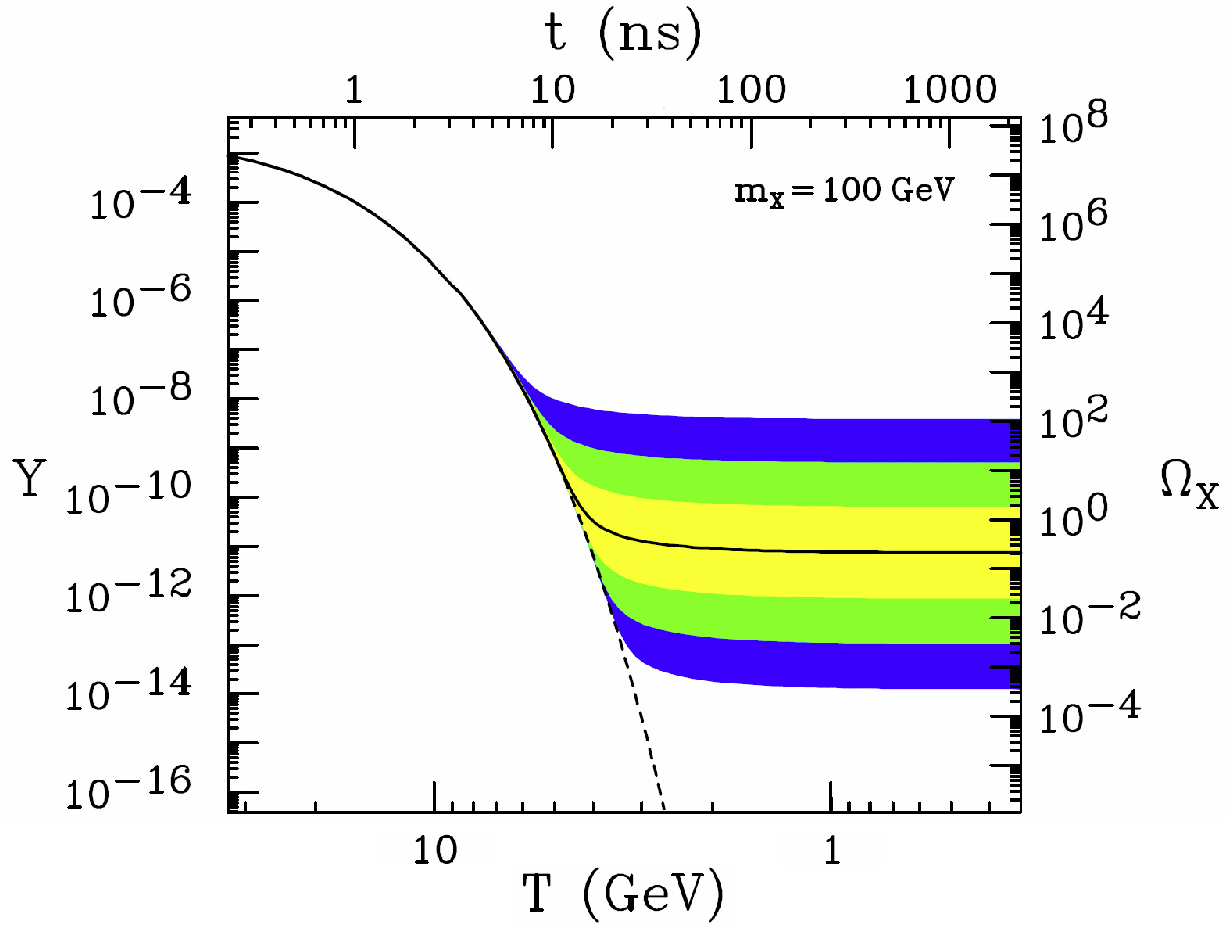
\includegraphics[scale=0.6]{Chapter_1/Figures/WIMP_Freezeout.pdf}
        \caption[Typical evolution of the WIMP number density in the early universe during the epoch of WIMP chemical freeze-out.]%
        {The plot represents the change in WIMP yield $Y$ as a result of the temperature $T$ in the early universe, which is equivalent to time $t$, governing the rate of expansion. The yellow, green and blue shaded regions represent the impact of changing the cross-section by a factor of $10$, $10^{2}$ and $10^{3}$ respectively \cite{Feng_2010}}.
        \label{fig:wimp_density_evolution}
        \end{center}
\end{figure}

As shown in the figure above, as the temperature approaches the freeze-out temperature ($T_{fo}$)---the point in which WIMPs are chemically decoupled---the annihilation rate becomes of the order of the Hubble expansion rate and the WIMP production becomes negligible, bringing the WIMP abundance per comoving volume to a constant value. The freeze-out temperature can be generalised as $T_{fo} \simeq m_\chi/20$ for varying WIMP masses and the velocity at which this freeze-out is reached calculated by $v_{fo} = (3T_{fo}/2m_{\chi})^{1/2} \simeq 0.27c$. The WIMP relic density, as illustrated above is inversely proportional to the annihilation cross-section and is independent of the WIMP mass. Smaller annihilation cross-sections lead to a larger relic density. Remarkably, an annihilation cross-section of an order of magnitude lower than that of the weak force will allow the relic density to match the current value of $\Omega_{CDM}$ as stated from cosmological observations. This rather unexpected connection between particle physics and cosmology has been commonly referred to as the “WIMP miracle”.


\subsubsection{WIMP Candidates}
\label{subsubsec:wimp_candidates}

One of the most favoured candidates for a WIMP comes from a Supersymmetry (SUSY) model called the Minimal Super-symmetric Standard Model (MSSM). MSSM is an extension of the Standard Model that introduces a new global symmetry between fermions and bosons. As well as containing all of the known fields of the standard model, the theory requires partners to form supersymmetric multiplets. These partners are associated as a "superpartner" for each particle of the Standard Model, which has the same internal quantum number apart from spin that differs by one half. Hence, every boson has a supersymmetric fermion partner while every fermion has a boson superpartner. 

The most important ingredient for supersymmetric dark matter is the newly defined global symmetric of SUSY called R-parity, expressed as \cite{Jungman_1996},
%
\begin{equation} \label{eq:r_parity}
    R = (-1)^{3(B-L) + 2S}
\end{equation}
%
where $B$, $L$ are the baryon and lepton number operators and $S$ is the spin. The R parity in this model produces the Standard Model particles for $R=+1$ and their supersymmetric partners for $R=-1$. The conservation of this new symmetry dictates that there must always be two SUSY particles in the vertices that contain them and annihilation or creation can occur only within pairs. If R parity is broken, there are no special rules to present the supersymmetric partners to decay with masses of order a few GeV or larger. This leads to the decay of heavier SUSY particles into lighter ones until they are locked in as a Lightest Supersymmetric Particle (LSP), which cannot decay further due to the conservation of energy. The LSP is, thus, stable and also being colourless and of neutral charge makes it an ideal dark matter candidate.

At low energies, there are four neutralinos that are fermions and are electrically neutral, the lightest neutralino ($\tilde{\chi}^{0}_{1}$) is stable in an R-parity conserved scenario of MSSM and the search for neutralinos are of interest in many accelerator searches \cite{Athron_2019}. Having been created in the early universe along with other SUSY particles, neutralinos are believed to exist in abundance to account for the missing matter content of the universe and hence is good candidate for WIMP dark matter. 


%%------------------------------$$
\section{Detection of WIMP Dark Matter}
\label{sec:candidates}

The phenomenological landscape of particle dark matter gives rise to many candidates, some of which are mentioned in section (\ref{sec:candidates}). This translates to a vast range of experimental techniques and methodologies in searching for these dark matter candidates, predominantly governed by the interaction mechanics of the proposed candidates. The nature of WIMP dark matter as postulated in section (\ref{subsubsec:motivation_wimps}) provides three search avenues: direct detection, indirect detection and production. Focus of many indirect searches are geared towards detecting annihilation events of dark matter candidates in galaxies, such as gamma rays, neutrinos, positrons, or anti-protons. Particle collider searches are aimed at producing dark matter via SM collisions and looking for missing transverse energy event topologies, as dark matter particles are expected to leave the detector undetected. The main topic of this section however is the direct detection of galactic dark matter particles that are present in the Milky Way galaxy.


\subsection{Local WIMP Halo Kinematics}
\label{subsec:halo}

\subsubsection{Local WIMP Density}
\label{subsec:DM_Density}

The density and distribution of dark matter in the Milky Way provide critical information on the dynamics of our galaxy and are particularly important for both direct and indirect dark matter searches. The local WIMP density ($\rho_0$) is an average over a volume of few hundred parsecs around the solar radius $R_o = (8.0 \pm 0.5) \; \MathText{kpc}$ \cite{galaxy_center_distance}. The differential event rate is directly proportional to the expected density, hence any observational uncertainty in $\rho_0$ translates into an uncertainty in the event rate and the inferred constraints on the measured scattering cross-section.

The exclusion limits calculated by many direct detection experiments use a canonical local WIMP density of $\rho_0 = 0.3 \; \MathText{GeV cm}^{-3}}$ to allow for easy comparison between different results. Although the estimations of this parameter has fluctuated over the past few decades, most estimates are of order two in agreement with one another \cite{Read_2014}. Some of the more recent calculations using the second data release from the Gaia space mission \cite{Gaia_2018} place the DM density at around $\rho_0 \simeq 0.47 \; \MathText{GeV cm}^{-3}}$, highlighting the sensitivity of this parameter on the methodology and the data-sets used in determining the local density \cite{Sivertsson_2018}.

\subsubsection{WIMP Velocity Distribution}
\label{subsec:WIMP_velocity}

Another quantity from the phase space distribution of DM that impacts the constraints on dark matter mass models of the Milky Way are the local circular speed $v_{c}$ and the escape velocity $v_{esc}$. The conventional approach used in calculating exclusion limits on signals, assumes an isotropic, spherically symmetric Maxwellian velocity distribution, known as the Standard Halo Model (SHM) and is given by,
%
\begin{equation} \label{eq:dm_velocity_distribution}
    f(\boldsymbol{v}) = \frac{1}{(2\pi{}\sigma^{2})^{1/2}} \MathText{exp} \left( -\frac{|\boldsymbol{v}|^{2}}{2\sigma{}^2} \right),
\end{equation}
%
where the speed dispersion is related to the local circular speed by $\sigma = v_{c}\sqrt{3/2}$. The local circular speed is the measure of the Sun's velocity with respect to the center of our galaxy and is usually measured with respect to objects assumed to be at rest with the center \cite{Bovy_2012}. These methods yield velocities of $v_{c} = 218-246 \; \MathText{km s}^{-1}$ with the canonical taken as $v_{c} = 220 \; \MathText{km s}^{-1}$, yielding a $\sigma \simeq 270 \; \MathText{km s}^{-1}$ \cite{canonical_speed}. The local escape velocity of the galaxy has been calculated by sampling high velocity stars from the RAVE survey to be $v_{esc} = 544 \; \MathText{km s}^{-1}$ \cite{Smith_2007}.

In order to fully understand and map out the kinematics of the WIMP distribution as observed by a detector on earth, one has to also take into account the WIMP velocity distribution in the rest frame of the detector. This is achieved by carrying out a time-dependent Galilean transformation, where, 
%
\begin{equation} \label{eq:dm_velocity_distribution}
    \boldsymbol{v} \rightarrow \boldsymbol{\tilde{v}} = \boldsymbol{v} + \boldsymbol{v}_{E}(t).
\end{equation}
%
The velocity contributions from earths motion relative to the galactic rest frame, $\boldsymbol{v}_{E}(t)$ is a time dependent contribution to the overall velocity distributions with three sub-components: motion of the local standard of rest (LSP), given as $(0,v_{c},0) \; \MathText{km s}^{-1}$ for an axi-symmetric Milk Way; the Sun's peculiar motion with respect to the LSP, determined by observing motions of stars in the solar neighbourhood and is $\sim(10, 5.2, 7.2) \; \MathText{km s}^{-1}$ \cite{Dehnen_1998}; and the Earth's orbit about the Sun, $v_{E} = 29.8 \; \MathText{km s}^{-1}$, provided the ellipticity of the Earth's orbit and the non-uniform motion of the Sun is ignored.

Although these contributions all play a role in the signal models of direct detection experiments, the main characteristics of the WIMP signal can accurately be modeled by using only the motion of LSP. The other variables become important for time-dependent searches. Furthermore, in a scenario in which DM is observed by direct detection experiment, the accuracy and precision of the DM distribution and kinematics on Earth will require further investigation. 


\subsection{WIMP-Nucleon Scattering}
\label{subsec:scattering}

Provided that the Milky Way is populated by a WIMP dark matter halo as detailed in section (\ref{subsec:halo}), then the WIMP flux on Earth is of the order $(100 \; \MathText{GeV}/\MathText{m}_{\chi}) \times 10^5  \; \MathText{cm}^{-2} \MathText{s}^{-1}$. Even though WIMPs are postulated to interact only weakly with SM particles, the WIMP flux as dictated by the WIMP halo is sufficiently large enough for a potential detection of a small faction of these particles, as they elastically scatter off of atomic nuclei. Many direct detection experiments aim to detect the recoils of WIMPs via their nuclear recoil, and measure the rate, $R$, along with the energies, $E_{R}$, of these recoils to determine the nature of dark matter (as proposed in  \cite{Detectability_of_dm}).

The differential event rate of WIMPs with masses $m_{\chi}$, scattering off of atomic nucleus with mass $m_{N}$, usually expressed in terms of $\MathText{counts} \; \MathText{kg}^{-1} \; \MathText{days}^{-1} \; \MathText{keV}^{-1}$ (often referred to as dru), is given by \cite{Bertone_book},
%
\begin{equation} \label{eq:dm_velocity_distribution}
    \frac{dR}{dE_{R}} = \frac{\rho_{0}}{m_{N} m_{\chi}} \int_{v_{min}}^{\infty} vf(\boldsymbol{v}, t) \frac{d\sigma_{WN}}{dE_{R}}(v, E_{R}) \, dv, 
\end{equation}
%
where $\rho_{0}$ is the local WIMP density, $f(v)$ is the WIMP velocity distribution in the detector frame and $\frac{d\sigma_{WN}}{dE_{R}}(v, E_{R})$ is the WIMP-nucleus elastic scattering differential cross-section. The relative speed at which the scattering takes place is of the order $100 \; \MathText{km}^{-1} \; \MathText{s}^-1$, hence the WIMP-nucleus scattering occurs in a non-relativistic limit and results in recoil energies that are characterised in the center of mass frame, $\theta^{\ast}$,
%
\begin{equation} \label{eq:cm_wimp_energy}
    E_{R} = \frac{\mu^{2}_{N}v^{2}(1-cos(\theta^{\ast})}{m_{N}},
\end{equation}
%
where the reduced WIMP-nucleus mass is given by $\mu_{N} = m_{\chi}m_{N}/(m_{\chi} + m+{N})$. The total event rate given as per kilogram per day in a typical detector can then be calculated by integrating equation (\ref{eq:dm_velocity_distribution}) between the limits of the smallest recoil energy---resulting from the minimum WIMP speed $(v_{min} = \sqrt{(m_{N}E_{R})/(2\mu^{2}_{N}})$---and infinity, to give, 
%
\begin{equation} \label{eq:dm_velocity_distribution}
    R = \int_{E_{T}}^{\infty} \frac{\rho_{0}}{m_{N} m_{\chi}} \int_{v_{min}}^{\infty} vf(\boldsymbol{v}, t) \frac{d\sigma_{WN}}{dE_{R}}(v, E_{R}) \, dv, 
\end{equation}
%
where $E_{T}$ is the threshold energy as a result of the smallest recoil. Its important to note that in practice, most detectors will have a detector specific threshold which is almost always greater than the minimum detectable recoil. 

The particle physics and the interaction properties of the WIMP-nucleus scattering is encoded into the differential cross-section as part of the equation above. This is often calculated from the effective Lagrangian describing the interaction of the particular WIMP model with the quarks and the gluons in the nucleus. The hadronic matrix elements that entail the quark-gluon content of the nucleus is usually a large source of uncertainty. The WIMP-nucleus differential cross-section can further be represented as a two part differential, entailing the spin-dependent (SD) and the spin-independent (SI) contributions from the nucleus and by encoding the form factor, $F(E_{R})$, that depends on the momentum transfer, $q=\sqrt{2m_{N}E_{R}}$ and accounts for the suppression caused by the coherence loss for event rates of heavier nucleus or WIMPs. The generalised form of the WIMP-nucleus scattering cross-section is given by,
%
\begin{equation} \label{eq:dependent_and_independent}
    \frac{dR}{dE_{R}} = \frac{m_{N}}{2\mu^{2}_{N}v^{2}} \left(\sigma_{0}^{SD}F^{2}_{SD}(E_{R}) + \sigma_{0}^{SI}F^{2}_{SI}(E_{R})\right),
\end{equation}
%
where $\sigma_{0}^{SD/SI}$ represents the spin-dependent and spin-independent cross-sections at zero momentum transfer.

The difference between the spin-dependent and -independent processes are best understood by examining the WIMP-quark interactions at the Lagrangian level. The contributions that arise from the spin-dependent interactions are due to the axial-vector couplings, whereas the spin-independent contributions are from scalar and vector couplings to quarks.

\subsubsection{Spin-dependent Scattering}
\label{subsec:SI_scatter}

The spin-dependent contribution to the WIMP-nucleus differential cross-section arises from coupling of the WIMP field to the quark axial-vector current, $\bar{q}\gamma^{\mu}\gamma_{5}q$ \cite{Jungman_1996}. If for example the WIMP is a Majorana or Dirac fermion, such as the lightest neutralino in MSSM, the Lagrangian for the WIMP-nucleon axial-vector interaction can be represented as,
%
\begin{equation} \label{eq:axial_vector_lagrangian}
   \mathcal{L}_{A} \supset \alpha^{A}_{q} (\bar{\chi}\gamma^{\mu}\gamma_{5}\chi) (\bar{q}\gamma_{\mu}\gamma_{5}q). 
\end{equation}
%
The resultant spin-dependent WIMP-nucleus differential cross-section can be represented by taking into account the contribution of different quarks of the quark spin matrix elements to the angular momentum, that is related to the matrix elements of the axial-vector current in the nucleus and the total angular momentum $\boldsymbol{J}$ of the nucleus, to give,
%
\begin{equation} \label{eq:nuclear_matrix_element}
   	\left(\frac{d\sigma_{WN}}{dE_{R}}\right)_{SD} = \frac{16m_{N}}{\pi{}v^{2}}\Lambda^2G^{2}_{F}J(J+1)\frac{S(E_{R})}{S(0)}.
\end{equation}
%
where $G_{F}$ is the Fermi constant, $\boldsymbol{J}$ is total angular momentum of the nucleus, and $\Lambda$ is a quantity that represents the product of the contributions from different quarks of the proton ($a_{p}$) and the neutron (${a_n$) and the expectation value of the spin content of the proton or the neutron group in the nucleus ($\langle S_{p,n} \rangle$). $\Lambda$ is given as,
%
\begin{equation} \label{eq:Lambda}
   	\Lambda = \frac{1}{J}[a_{p} \langle S_{p} \rangle + a_{n} \langle S_{n} \rangle],
\end{equation}
%
where $a_{p}$ and $a_{n}$ is,
%
\begin{equation} \label{eq:Lambda}
   	a_{p} = \sum_{q=u,d,s} \frac{\alpha^{A}_{q}}{G_{F}\sqrt{2}}\Delta^{p}_{q}; \; \; \; a_{n} = \sum_{q=u,d,s} \frac{\alpha^{A}_{q}}{G_{F}\sqrt{2}}\Delta^{n}_{q},
\end{equation}
%
where the quantities $\Delta^{p,n}_{q}$ are related to the matrix element of the axial-vector current of the nucleon ($\langle n|\bar{q}\gamma_{\mu}\gamma_{5}q|n \rangle = 2s^{n}_{\mu}$); $s_{\mu}$ is the spin of the nucleon, and $\Delta^{p,n}_{q}$ are values obtained using experimental data on lepton-proton scattering or simple nuclear models.

The exact coupling of WIMPs to protons or neutrons is not known, and although in reality
there are probably contributions from the two types, it is standard to consider “proton-only”
and “neutron-only” interactions separately. Consequently, heavy isotopes with an odd
number of neutrons will have in general a much larger SD sensitivity to the WIMP-neutron
channel.


\subsubsection{Spin-independent Scattering}
\label{subsec:SI_scatter}

The spin-independent contribution to the WIMP-nucleus differential cross-section arises from coupling of the WIMP field to the scalar-scalar and vector-vector currents in the Lagrangian,
%
\begin{equation} \label{eq:scalar_vector_lag}
   \mathcal{L}_{SV} \supset \alpha^{S}_{q} \bar{\chi} \chi \bar{q}q \; + \; \alpha^{V}_{q} \bar{\chi} \gamma_{\mu} \chi \bar{q} \gamma^{\mu}q.
\end{equation}
%
Under the assumption of a neutralino WIMP, the neutralino-nucleon scattering will have contributions from the squarks and the Higgs exchange \cite{Jungman_1996}. By taking into account the contributions of the scalar-scalar and vector-vector interactions and the resultant matrix elements, the generalised spin-independent WIMP-nucleus scattering with both scalar and vector interactions would read,
%
\begin{equation} \label{eq:si_rate}
   	\left(\frac{d\sigma_{WN}}{dE_{R}}\right)_{SI} = \frac{2m_{N}}{\pi{}v^{2}}\left[[Zf^{p} + (A + Z)f^{n}]^2 + \frac{B^{2}_{N}}{256}\right] F^{2}(E_{R}).
\end{equation}
%
where $Z$ is the number of protons, $(A-Z)$ is the number of neutrons, $f_{p}$ and $f{n}$ are the effective WIMP-proton and WIMP-neutron couplings, and $F^2(E_{R})$ is the nuclear form factor for coherent interactions and is understood as a Fourier transformation of the nucleon density and is usually parameterized in terms of the momentum transfer \cite{nuclear_form_wimp}. The individual contributions from the scalar and vector couplings to the cross-section are given by,
%
\begin{equation} \label{eq:scalar_vector_contributions}
   	\sigma_{S,0} = \frac{4\mu^{2}_{N}}{\pi}[Zf^{p} + (A-Z)f^{N}]^2
\end{equation}
%
%
\begin{equation} \label{eq:scalar_vector_contributions}
   	\sigma_{V,0} = \frac{mu^{2}_{N}B^{2}_{N}}{64\pi}
\end{equation}
%
with,
%
\begin{equation} \label{eq:scalar_vector_contributions}
   	B^{2}_{N} \equiv \alpha^{V}_{u}(A+Z) + \alpha^{V}_{d}(A-Z),
\end{equation}
%
representing the contributions of the valence quarks.

In most instances, the WIMP coupling to the neutrons and protons is approximately equal, that ($f_{n} \approx f_{p}$) and thus the spin-independent contribution scales as the square of the number of nucleons ($A^2$), whereas the spin-dependent contribution is proportional to the nuclear angular momentum, $(J+1)/J$. Due to the much larger enhancement from $A^2$, the spin-independent searches for heavier targets such as germanium, iodide or xenon, where ($A>20$), dominate the the SUSY parameter space.

\subsection{Direct Detection Searches}
\label{subsec:direct_searches}

The fundamental principle behind direct detection experiments is to design an experiment that has the potential to detect the recoiling of dark matter particles that transverse through the Earth, as the Earth travels through the dark matter halo present in our galaxy. These searches rely on a non-zero weak interaction between WIMPs and nuclei present in the detector volume. The main modes of detecting such a recoil signal lies in the ability of the detector to detect either the scintillation, ionisation or heat (phonons) that dissipates into the detection volume as a result of a WIMP-nucleus interaction. Ever since its proposal \cite{Detectability_of_dm}, there has been many experimental concepts developed using different target nuclei and detection techniques to probe for WIMP dark matter. 

The recoil energies expected from WIMPs as specified in section (\ref{eq:cm_wimp_energy}) is $\mathcal{O}(10-100 \; \MathText{keV})$ and the expected rates in a typical detection volume for a WIMP mass of $\sim 100 \; \MathText{GeV/c}^2$ is $\leq 1 \; \MathText{event/kg/year}$ \cite{Baudis_2012}. To overcome the difficulty of detecting such rate events, many experiments aim to build detectors at ultra-low background levels, especially in regions of energy-space that overlay a WIMP signal; and often, install the detectors in deep underground facilities. To detect recoil energies at keV-scale or below, a combination of signals are often used in reconstructing the energy deposition from a recoil medium, i.e. scintillation light and ionisation, or other combinations. Such an approach can allow for experiments to distinguish between different interactions, such as electron recoils (ER) and nuclear recoils (NR) and improve 3D position reconstruction of events; all of which can be used to reduce background rates to lower levels. 

\subsubsection{Sodium-Iodide \& Cryogenic Detectors}
\label{subsec:other_detectors}

A popular avenue for dark matter detection has been the use of thallium-doped sodium iodide (NaI(TI)) crystals. Experiments such as DAMA/LIBRA make use of such crystals to avoid background discrimination by modelling and observing the expected annual modulation of dark matter due to Earth's motion around the Sun \cite{dama_libra, dama_libra_new}. To the surprise of the community, they have been detecting an annual modulation at $\sim12\sigma$, claiming this to be a dark matter signature. Its important to note that this signature has not been seen in other dark matter experiments that has probed much more of the signal phase-space of a possible WIMP. Experiments such as COSINE-100 \cite{cosine_100} and SABRA \cite{sabre} are building detectors with similar detection technology to probe the DAMA/LIBRA discovery claim and conclude the saga once and for all. 

Cryogenic detectors operating at near-zero kelvin temperatures EDELWEISS \cite{edelweiss}, CDMS \cite{cdms} and CRESST \cite{cresst} can use a different combination of signal channels to achieve event-by-event discrimination between nuclear and electron recoils. The EDELWEISS and CDMS experiments extract the ionisation and phonons produced in an interaction site, while the CRESST experiment relies on scintillation and phonons. One of the downfalls of such experiments is to grow radio-pure crystals at much larger scales, limiting their ability to probe dark matter at ever-more sensitive cross-sections, but are capable at probing WIMP masses at much lower energies by reducing their energy thresholds to sub-keV regimes, as demonstrated by the CRESST-III experiment \cite{cresst_3}. 

\subsubsection{Liquid Noble Gas Detectors}
\label{subsec:liquid_noble_gas}

The history of liquid noble gases as a media for scintillation in search for galactic dark matter spans across several decades. Over this period, the experiments in this domain has narrowed their speciality in focusing on liquid -xenon (LXe) and -argon (LAr), as primary media for detecting scintillation and ionisation from particle interactions. The ability to detect both scintillation and ionisation is a unique feature of these liquids, in comparison to various other detection media. The capacity to scale-up to large mass with relatively trivial technology, has made LXe and LAr popular targets for dark matter, solar neutrino and neutrinoless double beta decay experiments. 

The advantage of using LXe and LAr as a detection media lies on their ability to scintillate in the vacuum ultraviolet (VUV) at $\sim178$ nm and $\sim128$ nm, respectively, making it relatively easy to detect such photons using photo-multiplier tubes (PMTs). The first noble gas detectors run primary as single-phase detectors, making use of only the scintillation photons produced from interaction sites. Some of these experiments include the single-phase LXe ZEPLIN-I \cite{zeplin_1} and XMASS \cite{xmass} experiments, and the single-phase LAr DEAP/CLEAN \cite{deap} experiment. Although, running singe-phase experiments simplify detector design, they come at a cost of scientific performance. For LXe, this is primarily in the reduction of discrimination power between ER and NR events, as the ionisation signal can serve as a way to distinguish these two event types. Furthermore, both LXe and LAr will endure more background leakage as a result of worst position reconstruction, as the outer edges of the liquid-scintillator usually serve as a self-shielding layer for backgrounds coming off of the TPC and detector walls.

To overcome some of these limitations, dark matter searches with LXe detectors progressed towards dual-phase LXe time-projection chambers (TPCs). Experiments such as ZEPLIN-II/III \cite{zeplin2, zeplin3}, XENON \cite{xenon100} and PandaX \cite{pandax} used dual-phase chambers to extract both the scintillation (S1) and ionisation (S2) signals by the use of electric-fields. The scintillation photons were detected using PMTs and the ionisation electrons were drifted towards the surface of the LXe and extracted through a gas-phase to generate S2 photons through electroluminescence. This technique allowed for much better ER/NR discrimination and 3D position reconstruction, reducing backgrounds leaking into the WIMP nuclear recoil signal from both ERs and wall backgrounds, by precisely fiducialising the active LXe region into a virtual central detection region of lower background, effectively rejecting the background dominated regions of the LXe. Some of the leading exclusion limits in the search for SI-WIMP-nucleon cross-section are shown in figure (\ref{fig:general_si_wimp_limits}). These experiments can effectively probe WIMP masses spanning a range of $\mathcal{O}(1-1000 \; \MathText{GeV/c}^2)$. Limitations at low-masses are usually due to the S1 signal thresholds, where at least a single-photon S1 has to coincide with an S2 signal. At these low recoil energies, coincidence backgrounds due to PMT dark-count rates usually dominate and hence thresholds are usually set higher. 
%
\begin{figure}[ht!]
    \begin{center}
        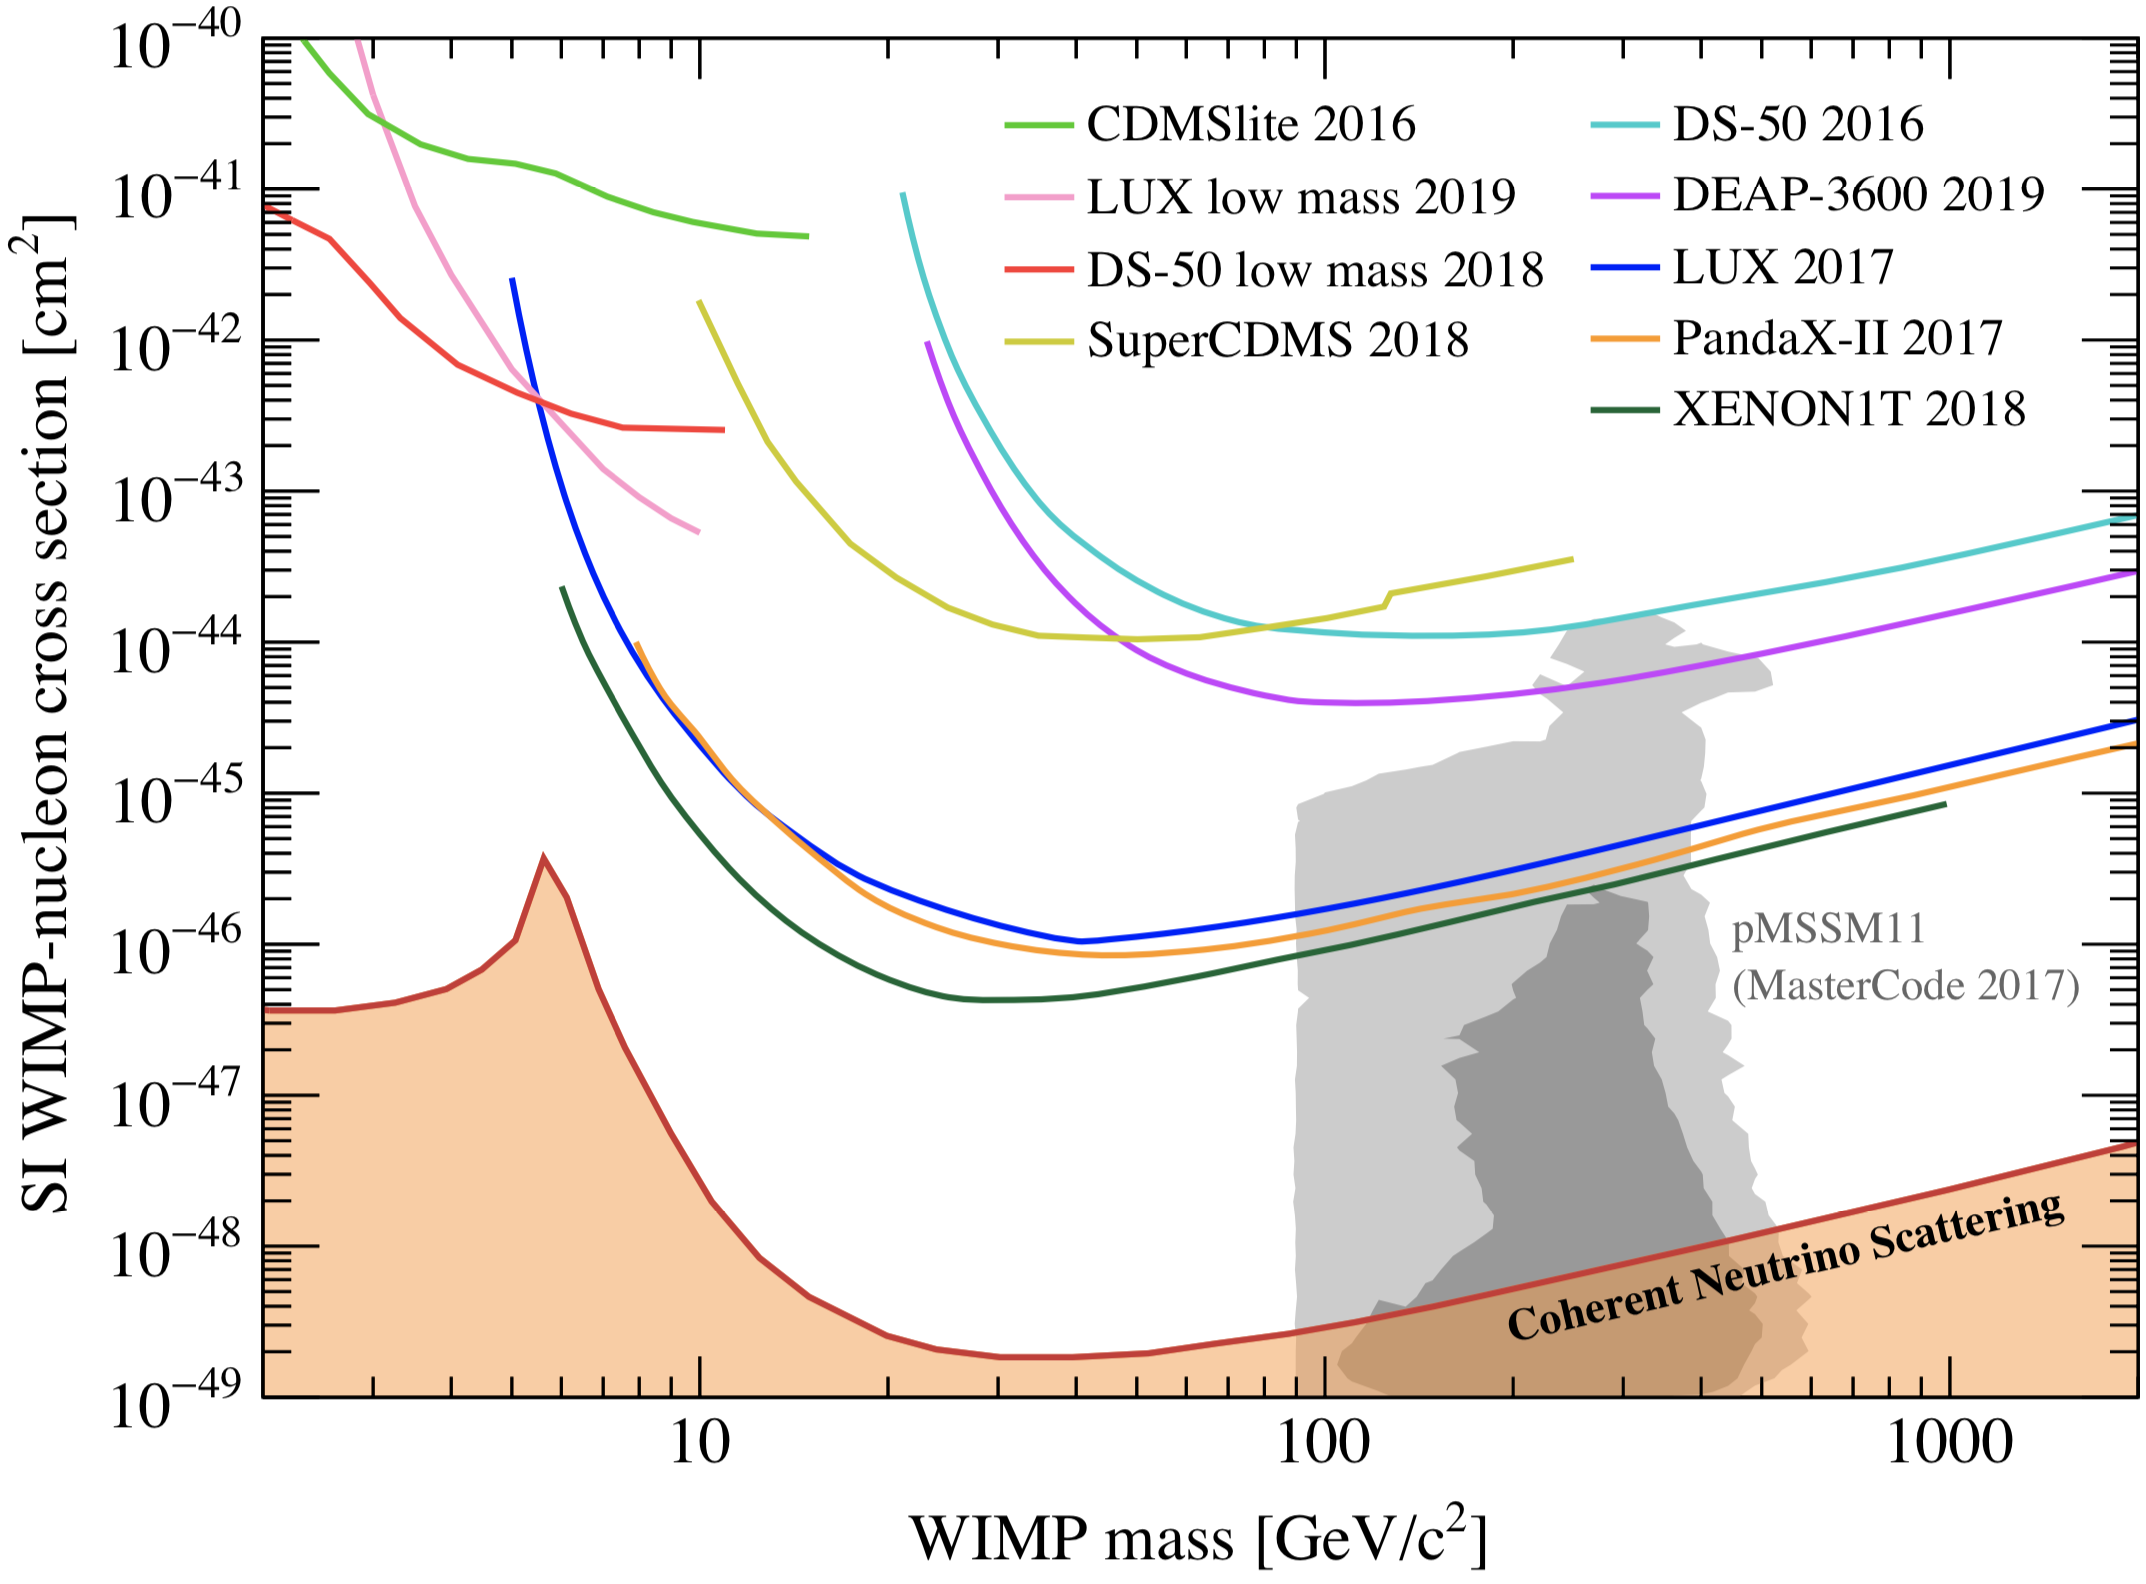
\includegraphics[scale=0.40]{Chapter_1/Figures/General_SI-WIMP_limits.png}
        \caption[Exclusion limits on the spin-independent WIMP-nucleon cross section as a function of WIMP mass from some of the leading direct detection experiments.]%
        {Spin-dependent WIMP-nucleon cross-section exclusion limits as a function of WIMP mass for some of the leading noble gas dark matter experiments and cryogenic crystal searches. The CDMSlite \cite{CDMS_2016} and the SuperCDMS \cite{CDMS_2018} limits are from cryogenic crystals. Low-mass WIMP analysis limits are from noble liquid detectors (\cite{lux_extended, darkside_50_lm}). And the remaining limits that span across most of the WIMP mass space are from liquid argon (\cite{DEAP_3600, darkside_50}) and liquid xenon (\cite{lux_full, xenon_1t, pandax_limit}) TPCs. The irreducible background from neutrinos, denoted as the \textit{neutrino floor} is shown as the brown shaded region \cite{neutrino_floor} and the $1\sigma$ and $2\sigma$ favoured contours from a recent global fit scan based on a pMSSM model are shown in grey \cite{pMSSM11}.}.
        \label{fig:general_si_wimp_limits}
        \end{center}
\end{figure}
%

